\documentclass{fhnwreport}         %[mode] = draft or final
%%---Main Packages-----------------------------------------------------------------------
\usepackage[english, ngerman]{babel}	%Mul­tilin­gual sup­port for LaTeX
\usepackage[T1]{fontenc}				      %Stan­dard pack­age for se­lect­ing font en­cod­ings
\usepackage[utf8]{inputenc}				  %Ac­cept dif­fer­ent in­put en­cod­ings
\usepackage{lmodern}                 %The newer Font-Set
\usepackage{textcomp}					      %LaTeX sup­port for the Text Com­pan­ion fonts
\usepackage{graphicx} 					      %En­hanced sup­port for graph­ics
\usepackage{float}						        %Im­proved in­ter­face for float­ing ob­jects
%\usepackage{ifdraft}                %Let you check if the doc is in draft mode

%%---Useful Packages---------------------------------------------------------------------
\usepackage[pdftex,dvipsnames]{xcolor}  %Driver-in­de­pen­dent color ex­ten­sions for LaTeX
\usepackage{csquotes}                   %Simpler quoting with \enquote{}
\usepackage{siunitx} 					     %A com­pre­hen­sive (SI) units pack­age
\usepackage{listings}					     %Type­set source code list­ings us­ing LaTeX
\usepackage[bottom]{footmisc}			  %A range of foot­note op­tions
\usepackage{footnote}					     %Im­prove on LaTeX's foot­note han­dling
\usepackage{verbatim}					     %Reim­ple­men­ta­tion of and ex­ten­sions to LaTeX ver­ba­tim
\usepackage[textsize=footnotesize]{todonotes} %Mark­ing things to do in a LaTeX doc­u­ment
\usepackage{lipsum}              % Gives you access to blindtext
\usepackage{booktabs,tabularx,array,csquotes}
\newcolumntype{Y}{>{\raggedright\arraybackslash}X} % Textspalte linksbündig, variabel
\newcolumntype{C}{>{\centering\arraybackslash}p{1.6em}} % schmale, zentrierte Spalte


%%---Tikz Packages-----------------------------------------------------------------------
%\usepackage{standalone}
%\usepackage{tikz}
%\usepackage{circuitikz}
%\usetikzlibrary{arrows}
%\usetikzlibrary{calc}
%\usetikzlibrary{intersections}

%%---Math Packages-----------------------------------------------------------------------
\usepackage{amsmath}					    %AMS math­e­mat­i­cal fa­cil­i­ties for LaTeX
%\usepackage{amssymb}					  %Type­set­ting symbols (AMS style)
%\usepackage{array}						  %Ex­tend­ing the ar­ray and tab­u­lar en­vi­ron­ments
%\usepackage{amsthm}					    %Type­set­ting the­o­rems (AMS style)

%%---Table Packages----------------------------------------------------------------------
\usepackage{tabularx}					  %Tab­u­lars with ad­justable-width columns
%\usepackage{longtable}
\usepackage{multirow}					  %Create tab­u­lar cells span­ning mul­ti­ple rows
\usepackage{multicol}					  %In­ter­mix sin­gle and mul­ti­ple columns

%%---PDF / Figure Packages---------------------------------------------------------------
\usepackage{pdfpages}					  %In­clude PDF doc­u­ments in LaTeX
\usepackage{pdflscape}					  %Make land­scape pages dis­play as land­scape
%\usepackage{subfig}					    %Fig­ures di­vided into sub­fig­ures

%%---Other Packages----------------------------------------------------------------------
%\usepackage{xargs}              %De­fine com­mands with many op­tional ar­gu­ments


%%---Main Settings-----------------------------------------------------------------------
\graphicspath{{./graphics/}}			%Defines the graphicspath
%\geometry{twoside=false}				%twoside=false disables the "bookstyle"
\setlength{\marginparwidth}{2cm}
\overfullrule=5em						    %Creates a black rule if text goes over the margins => debugging

%%---User Definitions--------------------------------------------------------------------
%%Tabel-Definitions: (requires \usepackage{tabularx})
\newcolumntype{L}[1]{>{\raggedright\arraybackslash}p{#1}}    %column-width and alignment
\newcolumntype{C}[1]{>{\centering\arraybackslash}p{#1}}
\newcolumntype{R}[1]{>{\raggedleft\arraybackslash}p{#1}}					                        %loads all packages, definitions and settings	

%%%%% Logo: Hocvhschule HTU oder HSI, Sprache DE oder EN:
\newcommand{\logofilename}{FHNW_HSI_DE}
\usepackage[style=apa,urldate=comp,backend=biber]{biblatex}
\usepackage{booktabs}
\usepackage{float} % für [H] bei Tabellen
\usepackage{booktabs}
\usepackage{float}
\usepackage[utf8]{inputenc}
\usepackage[T1]{fontenc}
\usepackage[ngerman]{babel}
\usepackage{booktabs}
\usepackage{float}
\usepackage{graphicx}
\addbibresource{literature/bib.bib}

\let\oldcite\cite
\renewcommand{\cite}{\parencite}
											
\title{The Architect's 1:1 Sandbox}  %Project Title
\author{Bachelor Thesis}    %Document Type => Technical Report, ...
\date{Windisch, August 2025}               %Place and Date

\begin{document}

\pagenumbering{roman}	

%%---TITLEPAGE---------------------------------------------------------------------------
\selectlanguage{ngerman}                  %ngerman or english
\maketitle

\begin{figure}[H]
\centering
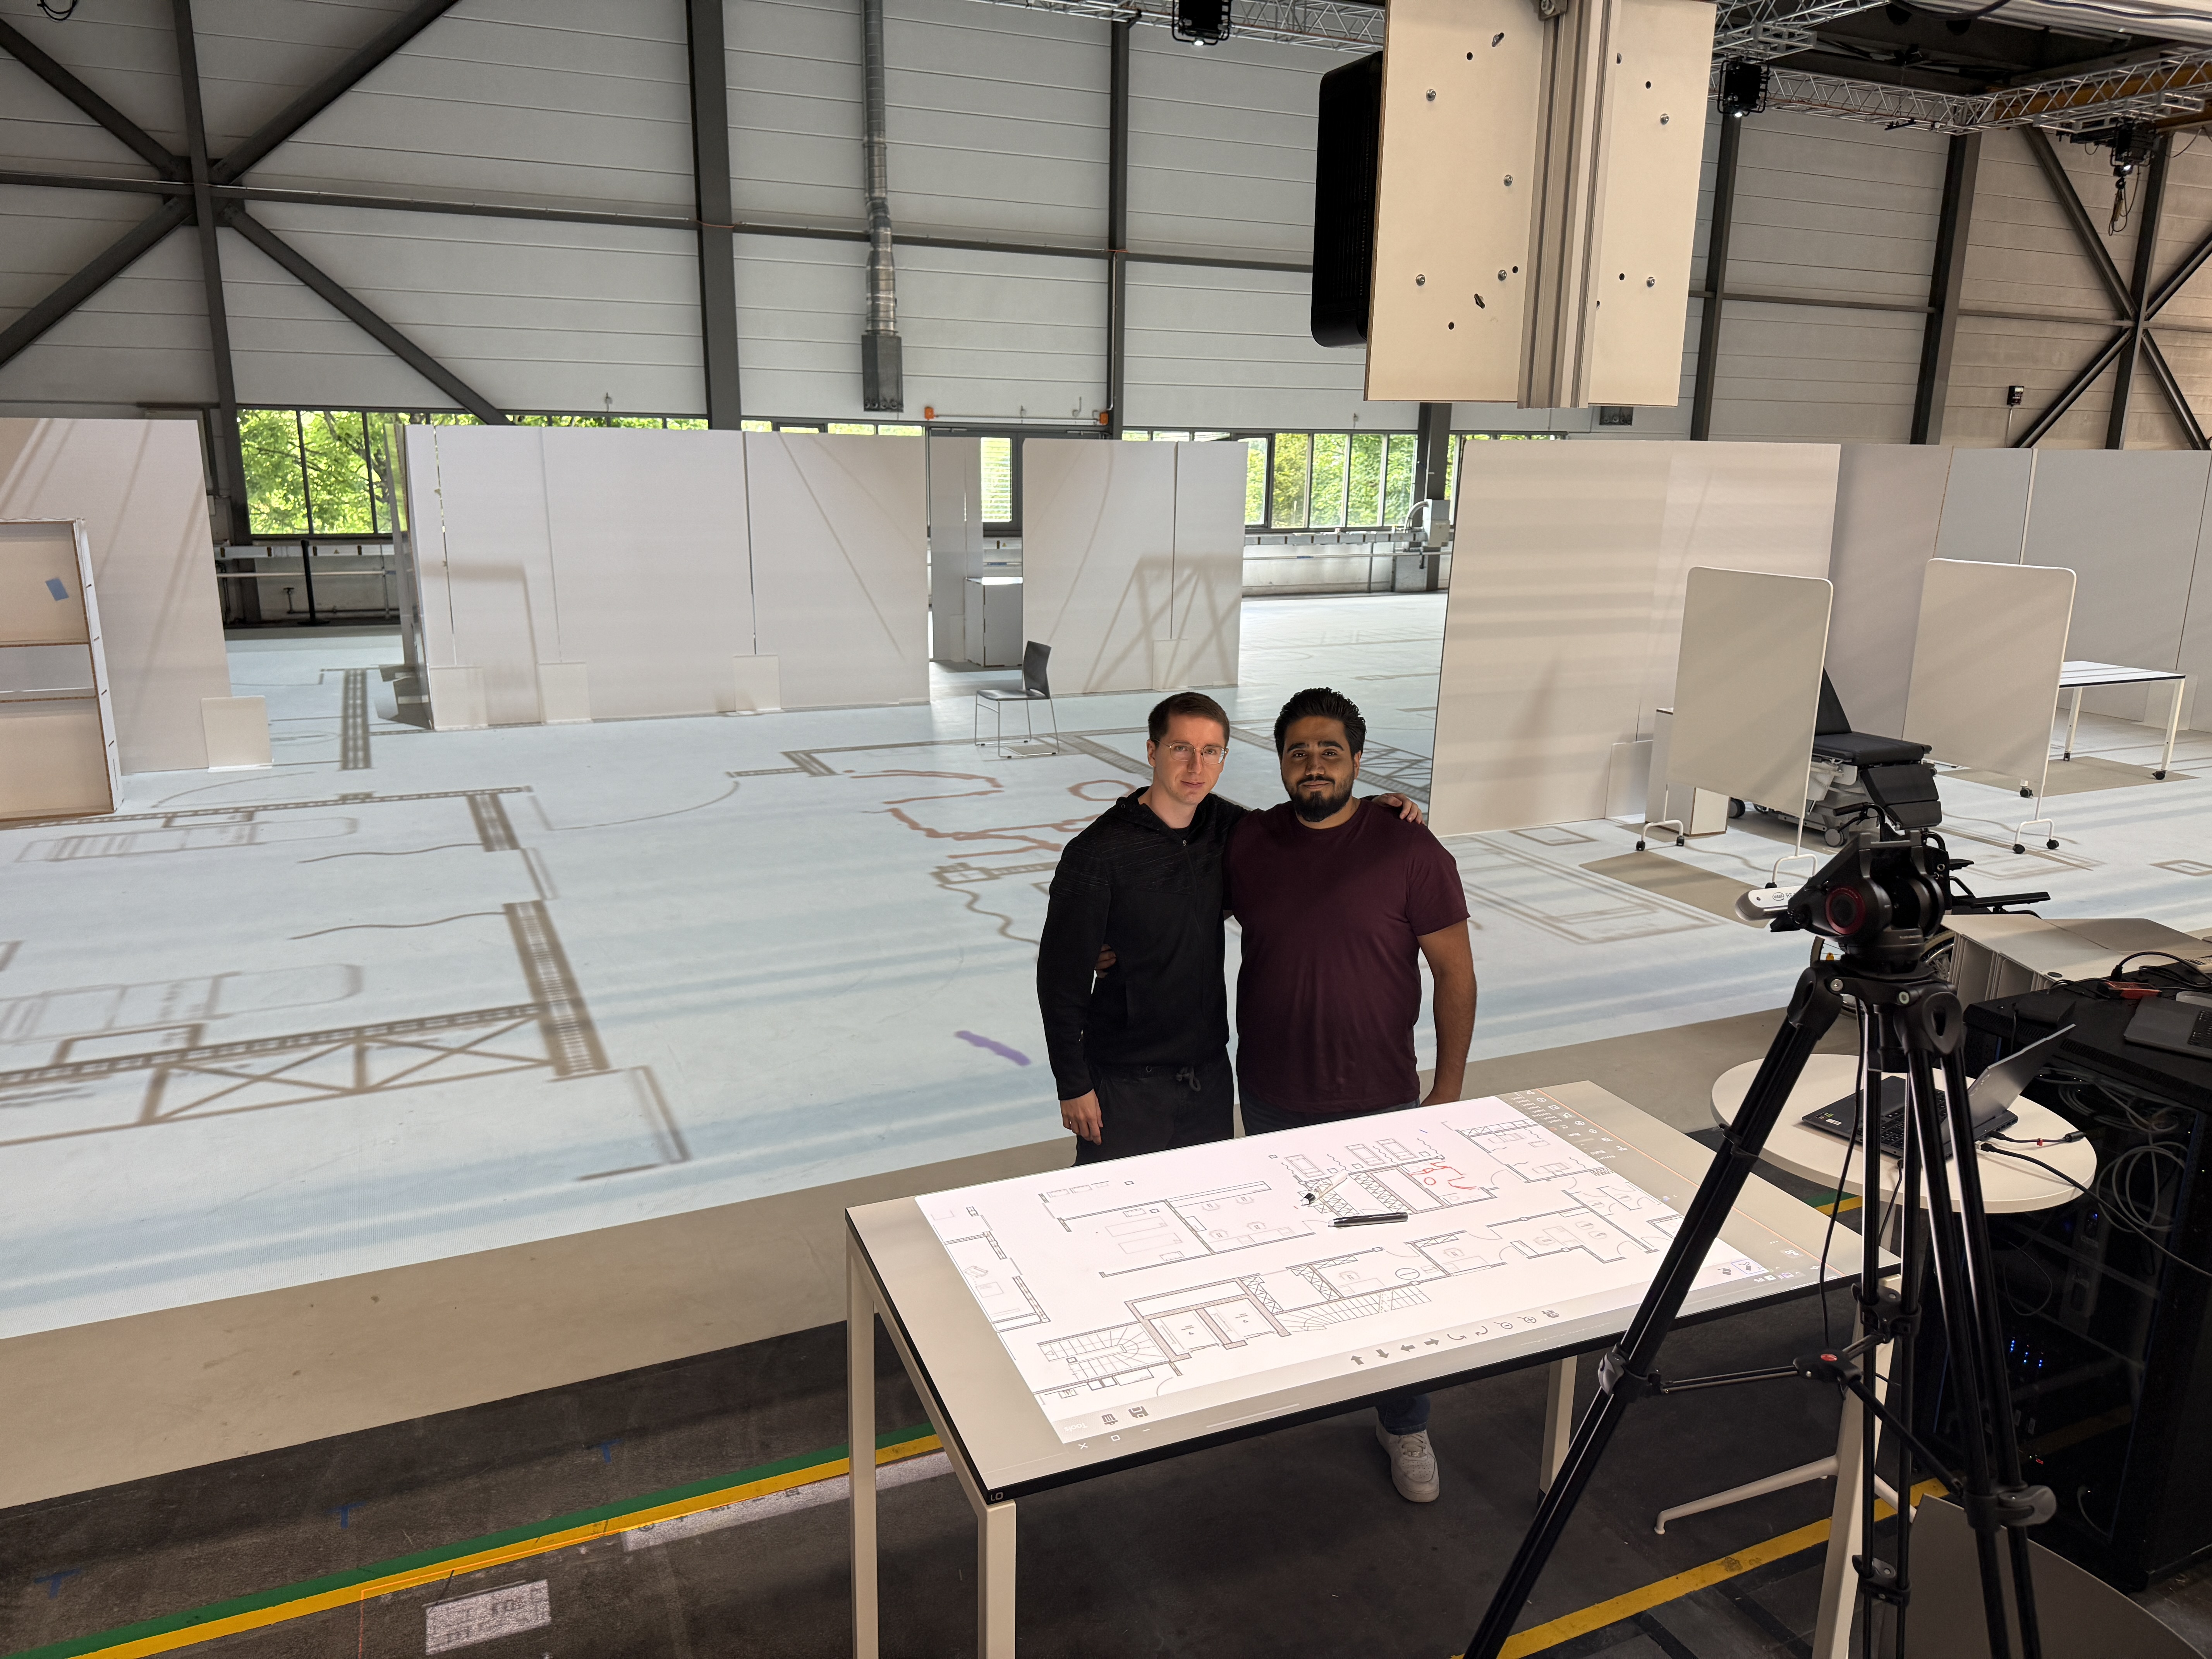
\includegraphics[width=0.8\linewidth]{graphics/titleimage.JPG}
\end{figure}

\vfill

\begin{tabular}{@{}p{5cm} l}
Studentin/Student          &    Luc Hartmann\\
                           &    Jasjot Singh\\[2ex]
Expertin/Experte           &    Reto Senn\\[2ex]
Betreuerin/Betreuer        &    Hilko Cords\\
                           &    Kevin Kim\\[2ex]
Auftraggeberin             &    SCDH\\[2ex]
Projektnummer              &    \verb|25FS_IIT41|\\[4ex]
\multicolumn{2}{@{}l}{Fachhochschule Nordwestschweiz, Hochschule für Informatik}
\end{tabular}

\vspace*{4ex}
% Beispiel für Logo Industriepartner
\begin{tikzpicture}[remember picture,overlay,every node/.style={anchor=north east}]
  \node at (current page.north east) [xshift=-1cm, yshift=-0.80cm] {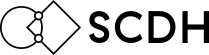
\includegraphics[width=4cm]{graphics/SCDH.png}};
  % Logo SCDH
\end{tikzpicture}


\clearpage
			
%%---ABSTRACT----------------------------------------------------------------------------
\selectlanguage{ngerman}				%ngerman or english
\thispagestyle{empty}
\section*{\centering{Abstract}}
Diese Bachelorarbeit beschreibt die Entwicklung eines digitalen Werkzeugs zur kollaborativen Grundrissgestaltung auf einer 1:1-Projektionsfläche. Ziel war es, eine benutzerfreundliche Anwendung zu realisieren, die insbesondere Laien in partizipativen Architektur-Workshops des Swiss Center for Design and Health (SCDH) unterstützt. Kern der Lösung ist ein interaktives Zeichenwerkzeug mit Infrarotstift-Tracking, dessen Position über eine Kamera erfasst und in Echtzeit auf die Projektionsfläche übertragen wird. Die Anwendung ermöglicht es mehreren Personen, simultan Raumkonzepte zu skizzieren, anzupassen und unmittelbar zu visualisieren.

Die plattformunabhängige Systemarchitektur wurde in praxisnahen Tests und einem Feldtest am SCDH evaluiert. Die Ergebnisse, darunter ein durchschnittlicher System Usability Scale (SUS)-Wert von 78.33 Punkten, bestätigen die intuitive Bedienbarkeit und den hohen Mehrwert für kollaborative Planungsprozesse. Damit leistet die Arbeit einen Beitrag zur Entwicklung niederschwelliger, technisch robuster Interfaces für die gemeinsame Raumplanung.



%%---TABLE OF CONTENTS-------------------------------------------------------------------	
\selectlanguage{ngerman}				%ngerman or english
\tableofcontents
\clearpage

\listoffigures
\listoftables
\cleardoublepage

%%---TEXT--------------------------------------------------------------------------------
\pagenumbering{arabic}
\section{Einleitung}
\label{einleitung}

Das Projekt \textit{The Architect's 1:1 Sandbox} wird im Auftrag des Swiss Center for Design and Health (SCDH) in Nidau durchgeführt. Das SCDH betreibt an seinem Standort in Nidau bei Biel eine Einrichtung, in der mittels Projektionen und Mockups Gebäudepläne im Massstab 1:1 dargestellt werden können. Diese Technologie ermöglicht die Erprobung von Abläufen und Prozessen sowie die Überprüfung von Designs in einer möglichst realitätsnahen Umgebung. Um dieses Angebot zu erweitern, soll im Rahmen des Projekts eine Softwarelösung entwickelt werden, die den initialen Gebäudedesign-Prozess vereinfacht und verbessert.

Ein zentrales Problem besteht darin, dass viele Personen keine Erfahrung im Gestalten von Gebäuden haben und dadurch während der ersten Bedarfsanalyse Schwierigkeiten bei der Formulierung und Visualisierung ihrer Anforderungen und Wünsche erleben. Das SCDH benötigt daher eine benutzerfreundliche Software, die es ermöglicht, gemeinsam mit den Kunden grobe Gebäudepläne zu erstellen und diesen ein besseres Verständnis sowie eine klare Übersicht über ihre Planung zu vermitteln.

Es existieren bereits einige CAD-Softwarelösungen zum Erstellen von Gebäudeplänen. Diese sind jedoch primär auf technische Detailplanung ausgerichtet und setzen gewisse Vorkenntnisse voraus. Zudem wurden sie selten für kollaborative Nutzung konzipiert, sondern meist für individuelle Arbeitsprozesse.

Das Ziel dieses Projekts ist die Entwicklung einer Softwarelösung, die auch Personen ohne Fachkenntnisse befähigt, funktionale Grundrissanordnungen zu entwerfen und dabei ein verständliches sowie anschauliches Bild der geplanten Räume zu erhalten. Die Zielgruppe ist somit relativ breit gefächert und umfasst alle, die ein Interesse an einer verbesserten Kommunikation und Visualisierung haben. Im Vordergrund steht eine benutzerfreundliche Gestaltung der Anwendung, die eine intuitive Bedienung ermöglicht und den Nutzenden in Kombination mit der 1:1-Projektionsfläche ein realistisches Raumgefühl vermittelt.

Die zu entwickelnde Software soll eine klare und nachvollziehbare Benutzeroberfläche bieten, die keine spezifischen architektonischen Vorkenntnisse voraussetzt. Sie soll es ermöglichen, individuelle Raumkonzepte mit Fokus auf Raumabfolgen und funktionale Zusammenhänge zu skizzieren. Dabei wird auf einfache Navigation, logische Strukturierung der Funktionen und unmittelbare Rückmeldung bei Eingaben besonderer Wert gelegt.

Ein wesentliches Merkmal der Lösung ist die Möglichkeit, Änderungen in Echtzeit vorzunehmen, die unmittelbar auf der 1:1-Projektionsfläche visualisiert werden. Dies soll auch eine kollaborative Arbeitsweise fördern, in der verschiedene Beteiligte wie Architekt:innen und Endnutzer:innen gemeinsam Planungen diskutieren und anpassen können.

Aus dieser Zielsetzung ergibt sich folgende Aufgabenstellung: Es soll eine flexible, intuitive und kollaborative Zeichenumgebung entstehen, die es ermöglicht, Bauelemente und Raumstrukturen in Echtzeit zu erfassen, zu bearbeiten und direkt zu projizieren. Eine mögliche Interaktionsvariante über ein kleineres Tischsystem mit synchronisierter Verbindung zur grossen Projektionsfläche wird ebenfalls in Betracht gezogen.

\clearpage

Im Rahmen des Projekts werden dazu drei zentrale \textbf{Forschungsfragen} untersucht, die die inhaltliche und gestalterische Entwicklung sowie die abschliessende Evaluation leiten:

\begin{enumerate}
    \item Wie können der Arbeitsablauf und das technische System gestaltet werden, damit Benutzer:innen kollaborativ an der einfachen und effizienten Planung von Grundrissen arbeiten können?
    \item Wie kann die Benutzeroberfläche so gestaltet werden, dass sie flexibel und funktionsreich ist, gleichzeitig aber auch für unerfahrene Nutzer:innen verständlich und intuitiv bleibt?
    \item Wie wird die vorgeschlagene Lösung von potenziellen Benutzer:innen hinsichtlich ihrer Benutzerfreundlichkeit und der Förderung der Zusammenarbeit wahrgenommen?
\end{enumerate}

Insgesamt zielt das Projekt darauf ab, eine benutzerzentrierte Lösung zu entwickeln, die die Komplexität der Gebäudeplanung reduziert, gleichzeitig aber ausreichend Flexibilität bietet, um individuelle Vorstellungen und Anforderungen umzusetzen. Dadurch soll die Software sowohl für private Bauherr:innen als auch für andere interessierte Gruppen ein nützliches Werkzeug zur interaktiven Planung und Visualisierung von Gebäuden darstellen.

\section{Hintergrund und verwandte Arbeiten}
\label{sec:Hintergrund und verwandte Arbeiten}

Dieses Kapitel gibt einen Überblick über die bestehenden Systeme zur Interaktion mit digitalen Zeichnungsumgebungen im Kontext der Raumplanung sowie über die technischen Grundlagen der entwickelten Lösung. Ziel ist es, die Relevanz des Projekts im bestehenden Lösungsraum aufzuzeigen und die Besonderheiten des eigenen Ansatzes zu motivieren. Zunächst wird der institutionelle Rahmen (SCDH) beschrieben, bevor im Anschluss technische Grundlagen, verwandte Systeme und der eigene Lösungsansatz vorgestellt werden.



\subsection{Projektkontext: Das SCDH und die bestehende Infrastruktur}

Das Projekt „The Architect's 1:1 Sandbox“ ist am Swiss Center for Design and Health (SCDH) in Nidau angesiedelt. Das SCDH betreibt eine Forschungsinfrastruktur, die es ermöglicht, Gebäudekonzepte im Massstab 1:1 mittels Projektoren und Mockups zu visualisieren. Diese Umgebung erlaubt es, architektonische Entwürfe gemeinsam mit Fachpersonen und Laien realitätsnah zu evaluieren und zu diskutieren.

Die Projektionsfläche des SCDH wird bislang primär verwendet, um bestehende Grundrisspläne darzustellen und physisch zu begehen. Interaktive Anpassungen oder kollaborative Zeichenvorgänge sind derzeit nur über analoge Mittel wie Papier oder Klebeband möglich. Die Integration einer digitalen Interaktionslösung stellt daher einen logischen nächsten Schritt zur Weiterentwicklung dieser Umgebung dar.

\begin{figure}[H]
    \centering
    \includegraphics[width=0.75\linewidth]{graphics/Bild_vorhandene_infrastruktur.JPG}
    \caption{Bestehende Anlage mit Mockup}
    \label{fig:placeholder}
\end{figure}

\clearpage

\subsection{Technologische Grundlagen}

Die Umsetzung basiert auf einem Infrarotstift, der eine punktuelle IR-Lichtquelle erzeugt, welche von einer externen Infrarotkamera (Intel RealSense D455) erfasst wird, in einem Outside-in-Tracking-Verfahren. Durch Segmentierung und Schwellenwertverfahren werden die hellsten Bildbereiche isoliert, um die Position der Stiftspitze zu bestimmen.

Mithilfe einer sogenannten Homographie-Matrix wird der erkannte Punkt aus dem Kamerakoordinatensystem in die Zeichenfläche transformiert. Dies ermöglicht eine präzise Interaktion auf einer beliebigen, zuvor kalibrierten Projektionsfläche. Die Kalibrierung erfolgt durch das gezielte Ansteuern vordefinierter Referenzpunkte, aus denen die Projektionsgeometrie berechnet wird.

Die gesamte Lösung ist so konzipiert, dass sie plattformunabhängig (Windows, macOS, Linux) funktioniert und sich flexibel an unterschiedliche Projektionssituationen anpassen lässt.

\subsubsection{Inside-out and Outside-in tracking}

\textbf{Inside-out:}
Beim Inside-out Tracking befindet sich die Sensorik, die für die Positionsbestimmung des Stiftes notwendig ist, direkt am Stift (oder dem Gerät, das den Stift trackt). Der Stift ''sieht'' von innen nach aussen in seine Umgebung und nutzt dort vorhandene Merkmale (z.B. optische Marker, natürliche Landmarken oder Inertialsensoren) zur Bestimmung seiner eigenen Position und Orientierung im Raum.\\
\cite{tracking_source}

\textbf{Outside-in:}
Beim Outside-in Tracking ist die Sensorik extern und fest in der Umgebung des Stiftes platziert (z.B. Kameras, Basisstationen). Diese externen Sensoren ''beobachten'' den Stift (oder Marker/Signale am Stift) von aussen und bestimmen dessen Position und Orientierung im Raum.\\
\cite{tracking_source}
\subsubsection{Infrarot}

Bei Infrarotstrahlung handelt es sich um einen Bereich des elektromagnetischen Spektrums direkt unterhalb des sichtbaren roten Lichts. Der Infrarotbereich umfasst Wellenlängen von etwa 780\,nm bis 1\,mm. Dieser Spektralbereich ist für das menschliche Auge unsichtbar. Für das vorliegende Projekt ist der sogenannte nahe Infrarotbereich von 780\,nm bis 3000\,nm relevant, da der eingesetzte Infrarotstift Licht im Bereich um 950\,nm emittiert.\\
\cite{optik_eugene_hecht}


\subsubsection{Homography}

Die Homographie beschreibt eine projektive Transformation zwischen zwei Ebenen und stellt ein zentrales Konzept in der Computer Vision sowie in der Photogrammetrie dar. Sie erlaubt es, die Abbildung von Punkten einer Bildebene auf eine andere zu modellieren, wobei Perspektivenverzerrungen berücksichtigt werden. Mathematisch wird eine Homographie durch eine 3×3-Matrix dargestellt, welche im homogenen Koordinatensystem operiert. Damit lassen sich Bildpunkte aus einer Perspektive so transformieren, dass sie der Sichtweise aus einer anderen Kameraposition entsprechen.
\\
\cite{cv_hartley_zisserman}

\clearpage

\subsubsection{Momente}

Momente sind ein statistisches Konzept, das auch auf Bildregionen und Bildobjekte angewendet werden kann. Sie beschreiben charakteristische Eigenschaften eines Objekts, wie etwa Lage, Grösse und Orientierung. In unserer Arbeit nutzen wir Momente, um den Schwerpunkt der erkannten Flächen zu bestimmen. Dieser lässt sich über folgende Formeln berechnen:

\[
x = \frac{M_{10}}{M_{00}}, \quad y = \frac{M_{01}}{M_{00}}
\]

\cite{momente}


\subsection{Vergleich möglicher Eingabemethoden}

Zur Auswahl der geeigneten Eingabetechnologie wurden drei Ansätze evaluiert: Lusee, Touchscreen und IR-Stift. Die folgende Übersicht erläutert die grundlegenden Eigenschaften dieser Systeme und vergleicht sie anhand zentraler Kriterien wie Latenz, Intuitivität, Kosten und Flexibilität.

\textbf{Lusee} ist ein ursprünglich an der FHNW entwickeltes System, das berührungslos mit Hilfe einer Kamera die Position eines Fingers erkennt. Die Interaktion erfolgt über Gesten auf einer Projektion. Obwohl das System intuitiv wirkt, leidet es unter hoher Latenz, eingeschränkter Präzision und begrenzter Flexibilität bei der Einrichtung.\\
\cite{lusee_hardware}

\textbf{Touchscreen-Systeme} ermöglichen eine sehr direkte und präzise Eingabe durch Berührung. Sie sind vielen Nutzer:innen vertraut und bieten eine hohe Reaktionsgeschwindigkeit. Allerdings sind grossflächige Touchsysteme teuer, schwer skalierbar und in Workshop-Setups (z.B. 1:1-Projektionen am Boden) nicht praktikabel.

\textbf{Der IR-Stift} erzeugt Infrarotlicht an der Spitze, das von einer externen Kamera (z.B. Intel RealSense D455) erkannt wird. Durch Kalibrierung und Bildverarbeitung lässt sich der Stift in Echtzeit zur Zeicheneingabe verwenden. Die Methode ist günstig, flexibel einsetzbar und für viele Nutzer:innen durch die Stiftmetapher leicht verständlich.

\begin{table}[H]
\centering
\caption{Vergleich verschiedener Eingabemethoden}
\label{tab:inputvergleich}
\begin{tabular}{lcccc}
\toprule
\textbf{System} & \textbf{Latenz} & \textbf{Intuitivität} & \textbf{Kosten} & \textbf{Flexibilität} \\
\midrule
Lusee & Hoch & Mittel & Gering & Gering \\
Touchscreen & Gering & Hoch & Hoch & Gering \\
IR-Stift (eigene Lösung) & Mittel & Hoch & Gering & Hoch \\
\bottomrule
\end{tabular}
\end{table}

\clearpage

\subsection{Begründung für die Wahl des IR-Stifts}

Der IR-Stift wurde schliesslich als bevorzugte Eingabemethode gewählt, da er eine für die meisten Nutzer:innen vertraute Stift-Metapher verwendet, eine hohe Genauigkeit ermöglicht und mit vergleichsweise geringem technischem Aufwand umsetzbar ist. Zudem erfordert er keine spezielle Berührungssensorik in der Zeichenfläche und ist somit besonders flexibel und portabel einsetzbar.

Die Integration in das geplante Tisch-Setup ist unkompliziert und unterstützt eine gleichberechtigte, kollaborative Nutzung durch mehrere Personen im Raum. Auch unter budgetären Bedingungen stellt diese Variante eine praktikable und nachhaltige Lösung dar.

Die Entscheidung für den IR-Stift wurde zudem mit dem Kunden abgestimmt, der die Begründung nachvollziehen konnte und ihr zustimmte.

\subsection{Vergleich bestehender Systeme}

Es existieren verschiedene Systeme zur berührungslosen oder berührungsbasierten Interaktion mit digitalen Flächen. Zu den wichtigsten gehören:

\begin{itemize}
  \item \textbf{BenQ PointWrite:}\\
  BenQ PointWrite ist eine kommerzielle Lösung von BenQ. Das System ist grundsätzlich interessant, jedoch im Vergleich zu nicht kommerziellen Lösungen sehr kostspielig und bei Schweizer Händlern nicht direkt verfügbar. Eine weitere Einschränkung besteht in der zwingenden Bindung an BenQ-Hardware, was die Flexibilität des Systems erheblich reduziert.\\
  \cite{benq_pointwrite}
  \begin{figure}[H]
      \centering
      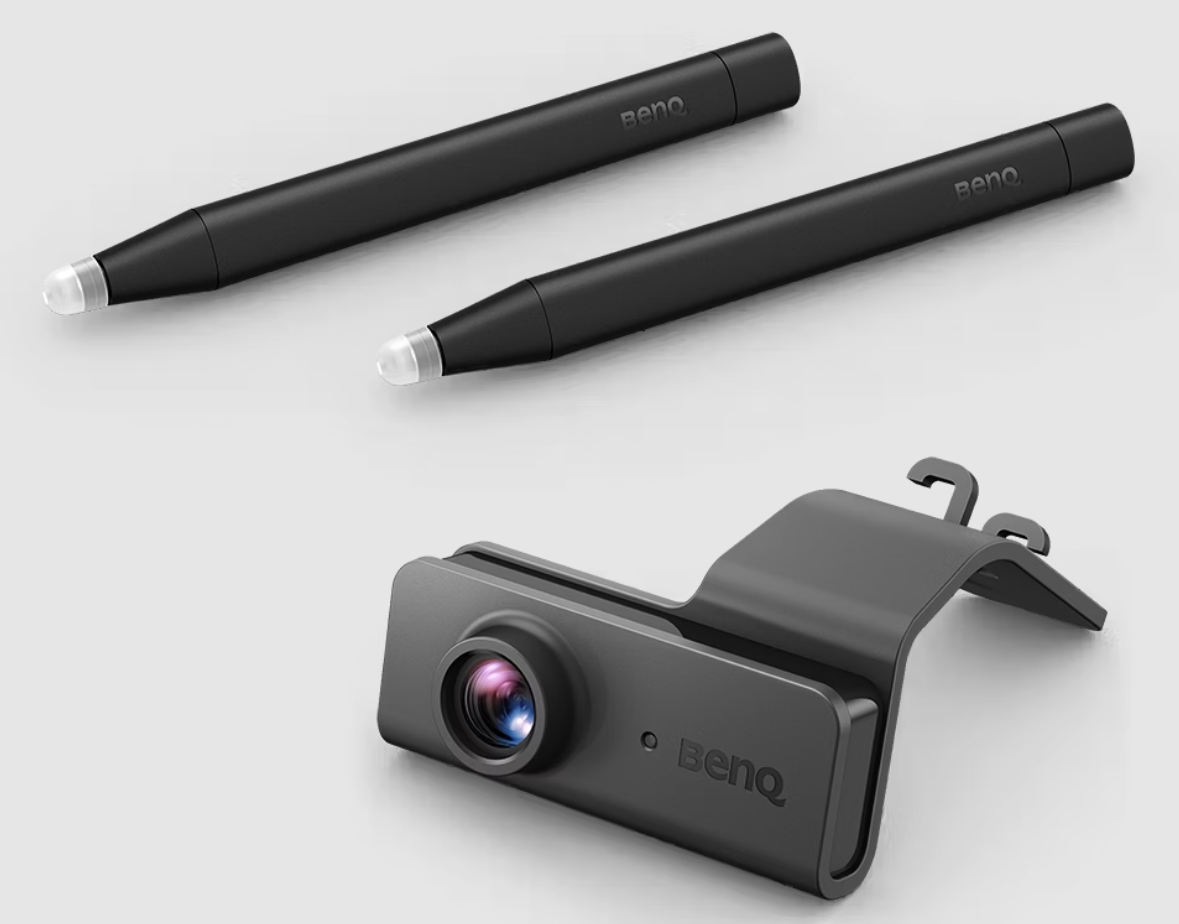
\includegraphics[width=0.5\linewidth]{graphics/benq.png}
      \caption{BenQ PointWrite}
      \cite{benq_pointwrite}
      \label{fig:benq_pointwrite}
  \end{figure}
  \clearpage

  \item \textbf{Nintendo Wii Remote (Wiimote):}\\
  Das Wiimote-Projekt ist ein bereits älteres Konzept, das einen Nintendo-Wii-Controller als Infrarotkamera verwendet. Positiv hervorzuheben sind die sehr kostengünstige Hardware und die einfache Handhabung des Systems. Problematisch ist jedoch, dass das System veraltet ist und keinen offiziellen Support mehr geniesst. In Verbindung mit der nicht mehr produzierten Hardware und veralteten Software wurde dies von uns als kritisch bewertet. Zudem kann ein Wii-Controller nur maximal vier Punkte gleichzeitig erfassen, wodurch die Anzahl gleichzeitiger Nutzer:innen auf höchstens vier begrenzt ist.\\
  \cite{wiimote}
  \begin{figure}[H]
      \centering
      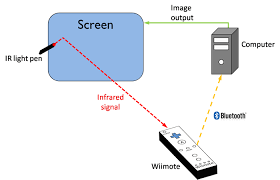
\includegraphics[width=0.5\linewidth]{graphics/wiimote.png}
      \caption{Grafische Übersicht der Wiimote}
      \cite{wiimote_image}
      \label{fig:wiimote}
  \end{figure}

  \item \textbf{Lusee (FHNW):}\\
  Bei Lusee handelt es sich um ein ehemaliges Projekt der FHNW, das inzwischen in eine eigenständige Firma übergegangen ist. Wir hatten die Möglichkeit, das System direkt an der FHNW zu testen. Es handelt sich um ein technisch interessantes Konzept mit einer ungewöhnlichen, aber innovativen Bedienung. Bei unserem Test fielen jedoch eine hohe Latenzzeit sowie gewisse Ungenauigkeiten negativ auf.\\
  \cite{lusee_hardware}
  \begin{figure}[H]
      \centering
      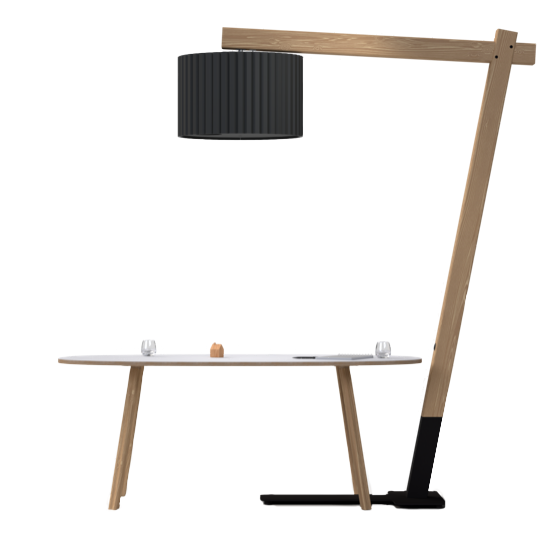
\includegraphics[width=0.4\linewidth]{graphics/lusee.png}
      \caption{Lusee}
      \cite{lusee_hardware}
      \label{fig:lusee}
  \end{figure}
\end{itemize}

\subsection{Einordnung des eigenen Ansatzes}

Wie Tabelle~\ref{tab:inputvergleich} zeigt, bietet der gewählte IR-Stift-Ansatz eine gute Balance zwischen Präzision, Kosten und technischer Einfachheit.

Im Gegensatz zu bestehenden Lösungen ist der eigene Ansatz:
\begin{itemize}
  \item kostengünstig und mit Standard-Hardware realisierbar,
  \item flexibel einsetzbar und plattformunabhängig,
\end{itemize}

Für den Ansatz mit einem IR-Stift bieten die bestehenden Lösungen derzeit kein zufriedenstellendes Angebot. Die Lösung von BenQ ist kostenintensiv und setzt den Einsatz proprietärer Hardware voraus. Das Wiimote-Projekt überzeugt zwar durch ein einfaches und kostengünstiges System, basiert jedoch auf veralteter Hardware und Software, die nicht mehr offiziell hergestellt oder unterstützt wird. Durch die Eigenentwicklung können wir die Lösung gezielt auf unsere spezifischen Anforderungen sowie auf die verfügbare Hardware abstimmen.
\section{Analyse der Ausgangslage}

Dieses Kapitel untersucht die konkrete Ausgangssituation, in der das Projekt verankert ist.  
Basierend auf einem Workshop am Swiss Center for Design and Health (SCDH) sowie der übergeordneten Zielsetzung werden zentrale Probleme und Anforderungen identifiziert, die für die Entwicklung der geplanten Softwarelösung relevant sind.  
Die im vorangegangenen Kapitel~\ref{sec:Hintergrund und verwandte Arbeiten} dargestellten technischen Grundlagen und bestehenden Systeme bilden dabei die Grundlage für die folgende Analyse.

Zunächst wird der beobachtete Workshopverlauf beschrieben, um die praktische Anwendungssituation besser zu verstehen. Anschliessend werden daraus konkrete Anforderungen abgeleitet, welche die technische und gestalterische Umsetzung im weiteren Projektverlauf mitprägen.


\subsection{Beobachtungen im Workshop}
\label{sec:workshop}

Im Rahmen des Projekts wurde ein Workshop des SCDH besucht, der am 3.~April~2025 in Nidau stattfand. Auftraggeber des Workshops war das Wohnheim Humanitas aus Horgen. Ziel war es, die geplanten Arbeitsabläufe im zukünftigen Neubau des Wohnheims im Zusammenhang mit einem Assistenzkran realitätsnah zu simulieren und zu evaluieren.

\begin{figure}[H]
  \centering
  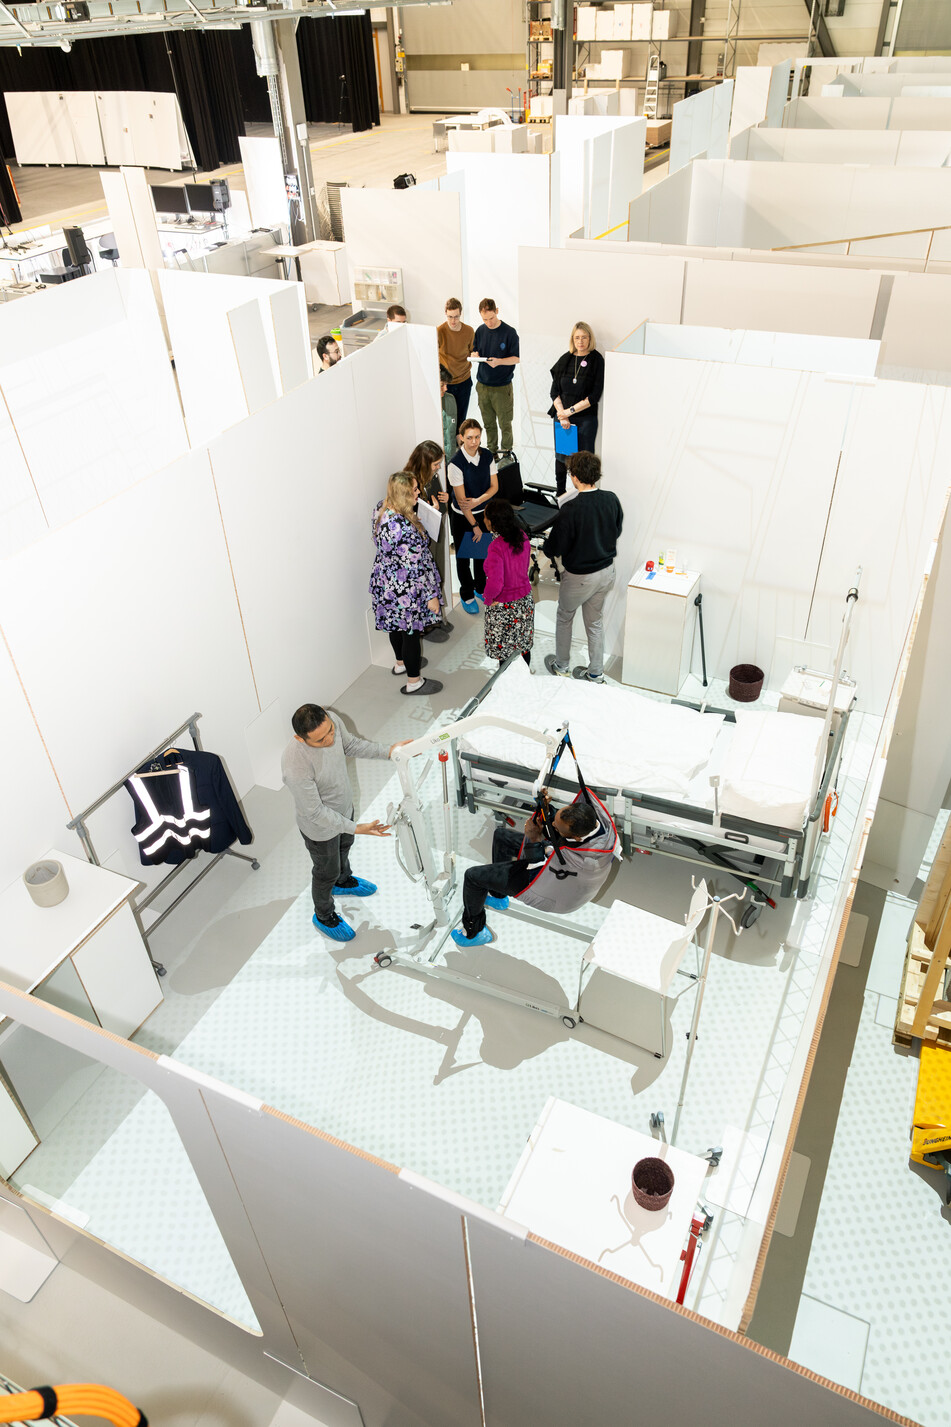
\includegraphics[width=0.5\linewidth]{graphics/workshop.jpg}
  \caption{Simulation der Barrierefreiheit im Neubau der Humanitas Stiftung}
  \cite{scdh_humanitas_image_nodate}
  \label{fig:humanitas_image}
\end{figure}
\clearpage


Hierzu wurden die bestehenden Baupläne auf die 1:1-Projektionsfläche überspielt. Das Workshopteam nutzte diese Fläche, um verschiedene alltägliche Situationen direkt vor Ort nachzustellen und auszuführen. Die Teilnehmenden konnten sich so durch Rollenspiel ein Bild von typischen Interaktionen und Bewegungsabläufen im geplanten Raumkonzept machen.

Der Ablauf des Workshops war in drei Phasen gegliedert:

\begin{itemize}
  \item \textbf{Briefing:} Gemeinsame Einführung in die Zielsetzung und den Planungsstand.
  \item \textbf{Simulation:} Aktives Begehen und Durchspielen der Szenarien auf der Projektionsfläche.
  \item \textbf{Debriefing:} Diskussion und Reflexion von Verbesserungsmöglichkeiten am Raumkonzept.
\end{itemize}

Besonderes Augenmerk lag auf den Phasen \textit{Briefing} und \textit{Debriefing}, da diese für das Projekt relevant sind: In diesen Momenten hätten digitale Zeichen- und Interaktionsmöglichkeiten den Austausch zwischen Teilnehmenden nachweislich unterstützen können (siehe auch Abschnitt~\ref{sec:verbesserungspotentiale}).



\subsection{Abgeleitete Anforderungen aus dem Workshop}

Die Beobachtungen vor Ort bestätigten nicht nur die Anforderungen aus der ursprünglichen Aufgabenstellung, sondern lieferten zusätzliche Einblicke in praktische Herausforderungen.

Folgende zusätzliche Anforderungen und Erkenntnisse wurden im Workshop identifiziert:

\begin{itemize}
  \item \textbf{Niederschwellige Bedienung:} Die Lösung muss auch von Personen ohne technische Vorkenntnisse oder mit sprachlichen Barrieren genutzt werden können.
  \item \textbf{Echtzeit-Funktionalität:} Änderungen müssen sofort sichtbar sein, um den Diskussionsfluss nicht zu unterbrechen.
  \item \textbf{Zugängliche Bedienung vom Platz aus:} Teilnehmende sollen Zeichnungen oder Korrekturen vornehmen können, ohne sich zur Projektionsfläche bewegen zu müssen.
  \item \textbf{Unterstützung spontaner Visualisierung:} Ideen und Probleme (z.\,B. Türrichtung, Gerätepositionierung) müssen spontan eingezeichnet werden können, um Missverständnisse zu vermeiden.
\end{itemize}

Diese Anforderungen belegen, dass ein interaktives Zeichensystem einen echten Mehrwert für solche Workshops darstellen kann, nicht nur zur Planung, sondern auch zur Verbesserung von Kommunikation, Teilhabe und gemeinsamen Entscheidungen.


\include{sections/Lösung}
\section{Implementation}
In diesem Kapitel wird die Architektur des Gesamtsystems sowie die Hardware- und Software-Implementierung beschrieben.

\subsection{Architektur}
Das System besteht aus einer in C\# entwickelten Software, der Infrarotkamera Intel RealSense D455 und einem generischen Infrarotstift. Die Software ist plattformübergreifend kompatibel mit Windows, Linux und macOS.

\begin{figure}[H]
    \centering
    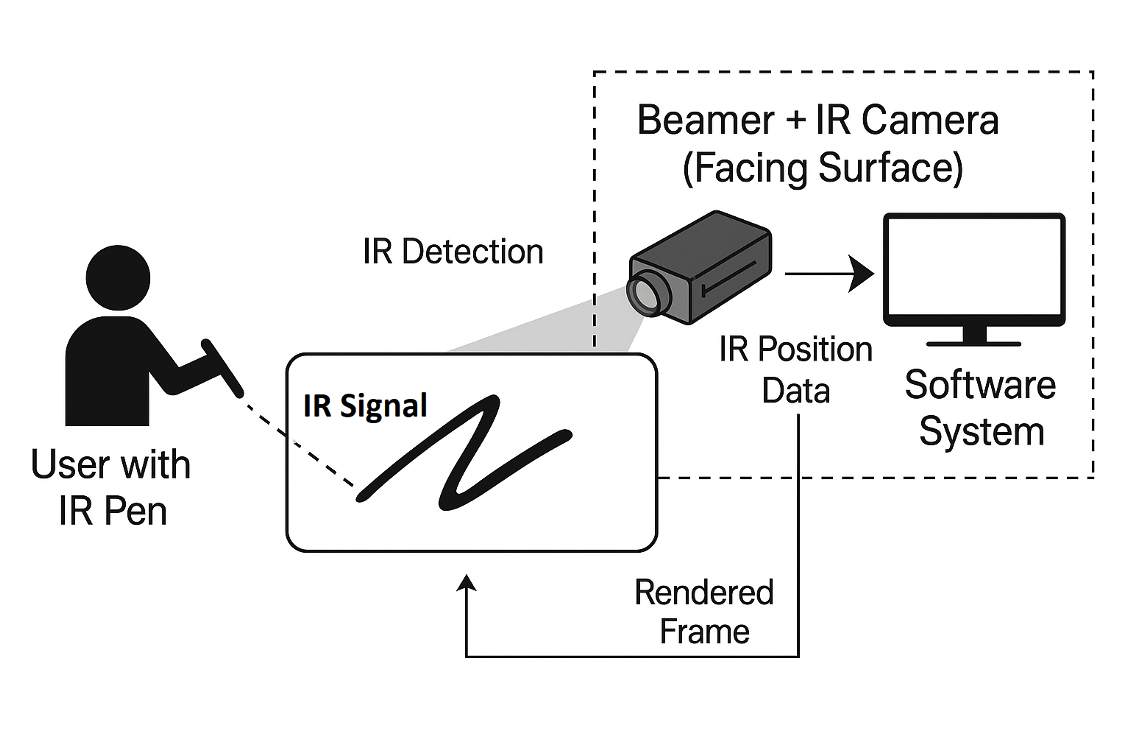
\includegraphics[width=0.5\linewidth]{graphics/system_uebersicht.png}
    \caption{Systemübericht}
    \label{fig:enter-label}
\end{figure}

\subsection{Setup}

Für das Setup muss die Kamera an den Computer angeschlossen und auf einen Bildschirm oder eine Projektionsfläche ausgerichtet werden. Anschliessend kann die Kalibrierung der Zeichenfläche über das Menü \texttt{Tools~→~Kalibrierung} (oben rechts in Abbildung \ref{fig:UI_screenshot}) gestartet werden. Im Kalibrierungsfenster muss der Infrarotstift nacheinander auf die fünf eingeblendeten Punkte gerichtet und aktiviert werden. Sobald sich das Fenster schliesst, ist das System bereit, um die Zeicheneingaben korrekt zu erfassen. Anschlissend können noch die PDF funktionen und die Gittergrösse angepasst werden.

\begin{figure}[H]
    \centering
    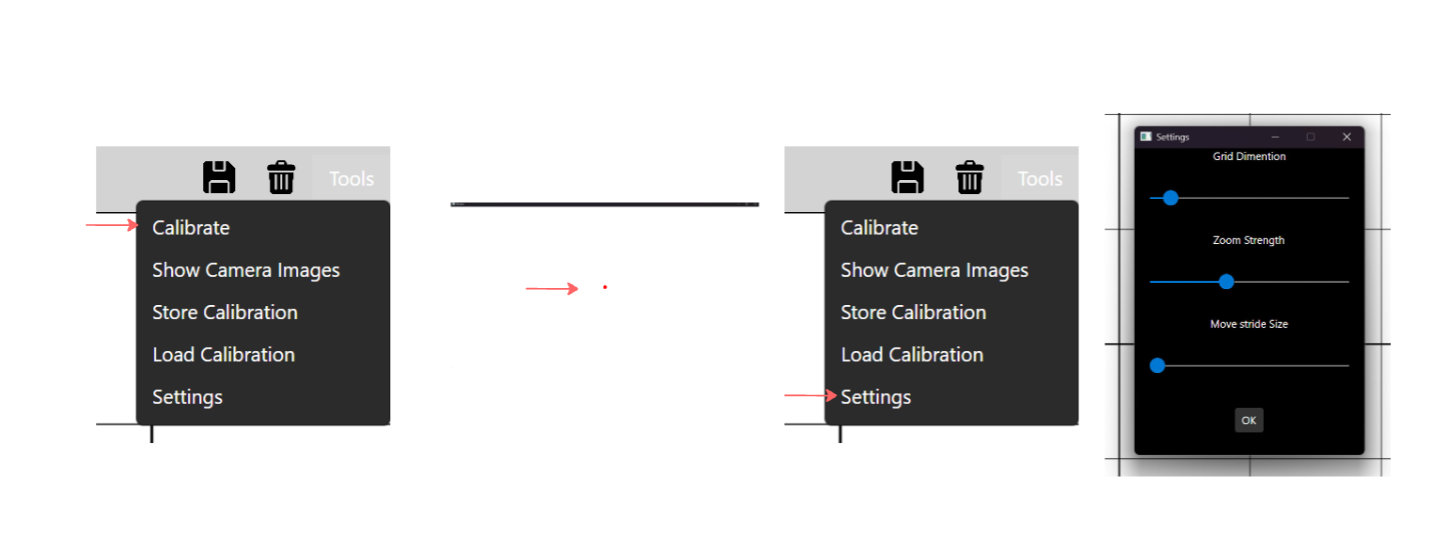
\includegraphics[width=0.8\linewidth]{graphics/anleitung_setup.png}
    \caption{Kurzanleitung für das Setup}
    \label{fig:anleitung_setup}
\end{figure}

Mit den Buttons Store- und Load Calibration kann die aktuelle Kalibration abgespeichert oder geladen werden um bei gleichem Setup die Einrichtung überspringen zu können.

\subsection{Hardware-Setup}
In diesem Abschnitt erläutern wir die eingesetzte Hardware sowie Anforderungen an mögliche Alternativen.

\vspace{0.5em}
\subsubsection{Infrarotstift}
Wir verwenden einen generischen Infrarotstift (siehe Anhang für Verkaufslink \ref{hw-info}). Dieser verfügt über eine Infrarot-LED, die durch das Eindrücken der Spitze oder das Drücken einer Taste auf der Oberseite aktiviert wird.

\begin{figure}[H]
    \centering
    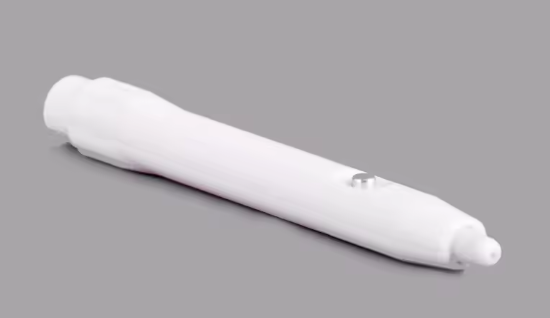
\includegraphics[width=0.5\linewidth]{bild_pen.png}
    \caption{Bild eienes Infrarotstiftes}
    \label{fig:enter-label}
\end{figure}

Es kann auch ein beliebiger anderer Infrarotstift verwendet werden. In der nachfolgenden Abbildung ist ein einfaches elektrisches Schema für die Mindestanforderung an die Hardware.

\begin{figure}[H]
    \centering
    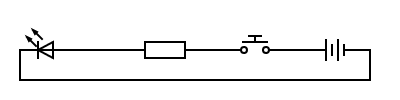
\includegraphics[width=0.5\linewidth]{schema_pen.png}
    \caption{Beispiel Schema für Infrarotstift}
    \label{fig:enter-label}
\end{figure}


\clearpage
%\vspace{0.5em}
\subsubsection{Infrarotkamera}

Wir verwenden die Infrarotkamera Intel RealSense D455, da sie dem SCDH bereits zur Verfügung stand. Die D455 verfügt über zwei Infrarotkameras, eine RGB-Kamera sowie einen steuerbaren Infrarot-Laser. Für unsere Anwendung genügt eine der beiden IR-Kameras.

\begin{figure}[H]
    \centering
    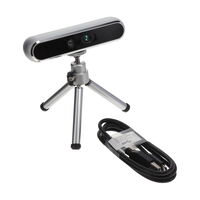
\includegraphics[width=0.5\linewidth]{graphics/bild_d455.jpg}
    \caption{Intel RealSense D455}
    \label{fig:enter-label}
\end{figure}

Zur Verbesserung der Bildqualität unter schwierigen Lichtverhältnissen wurde eine Filterfolie angebracht (Dämpfungskurve ersichtlich in Abbildung\ref{fig:filter_kurve}). Als Ersatz eignen sich prinzipiell alle Intel RealSense IR-Kameras mit SDK-Unterstützung. Mit Anpassungen in der InfraredCamera-Klasse können auch andere Kameramodelle eingesetzt werden.

\clearpage

\subsection{Software}
In diesem Abschnitt stellen wir zentrale Softwarekomponenten vor.

\vspace{0.5em}
\subsubsection{Benutzeroberfläche (UI)}
\begin{figure}[H]
    \centering
    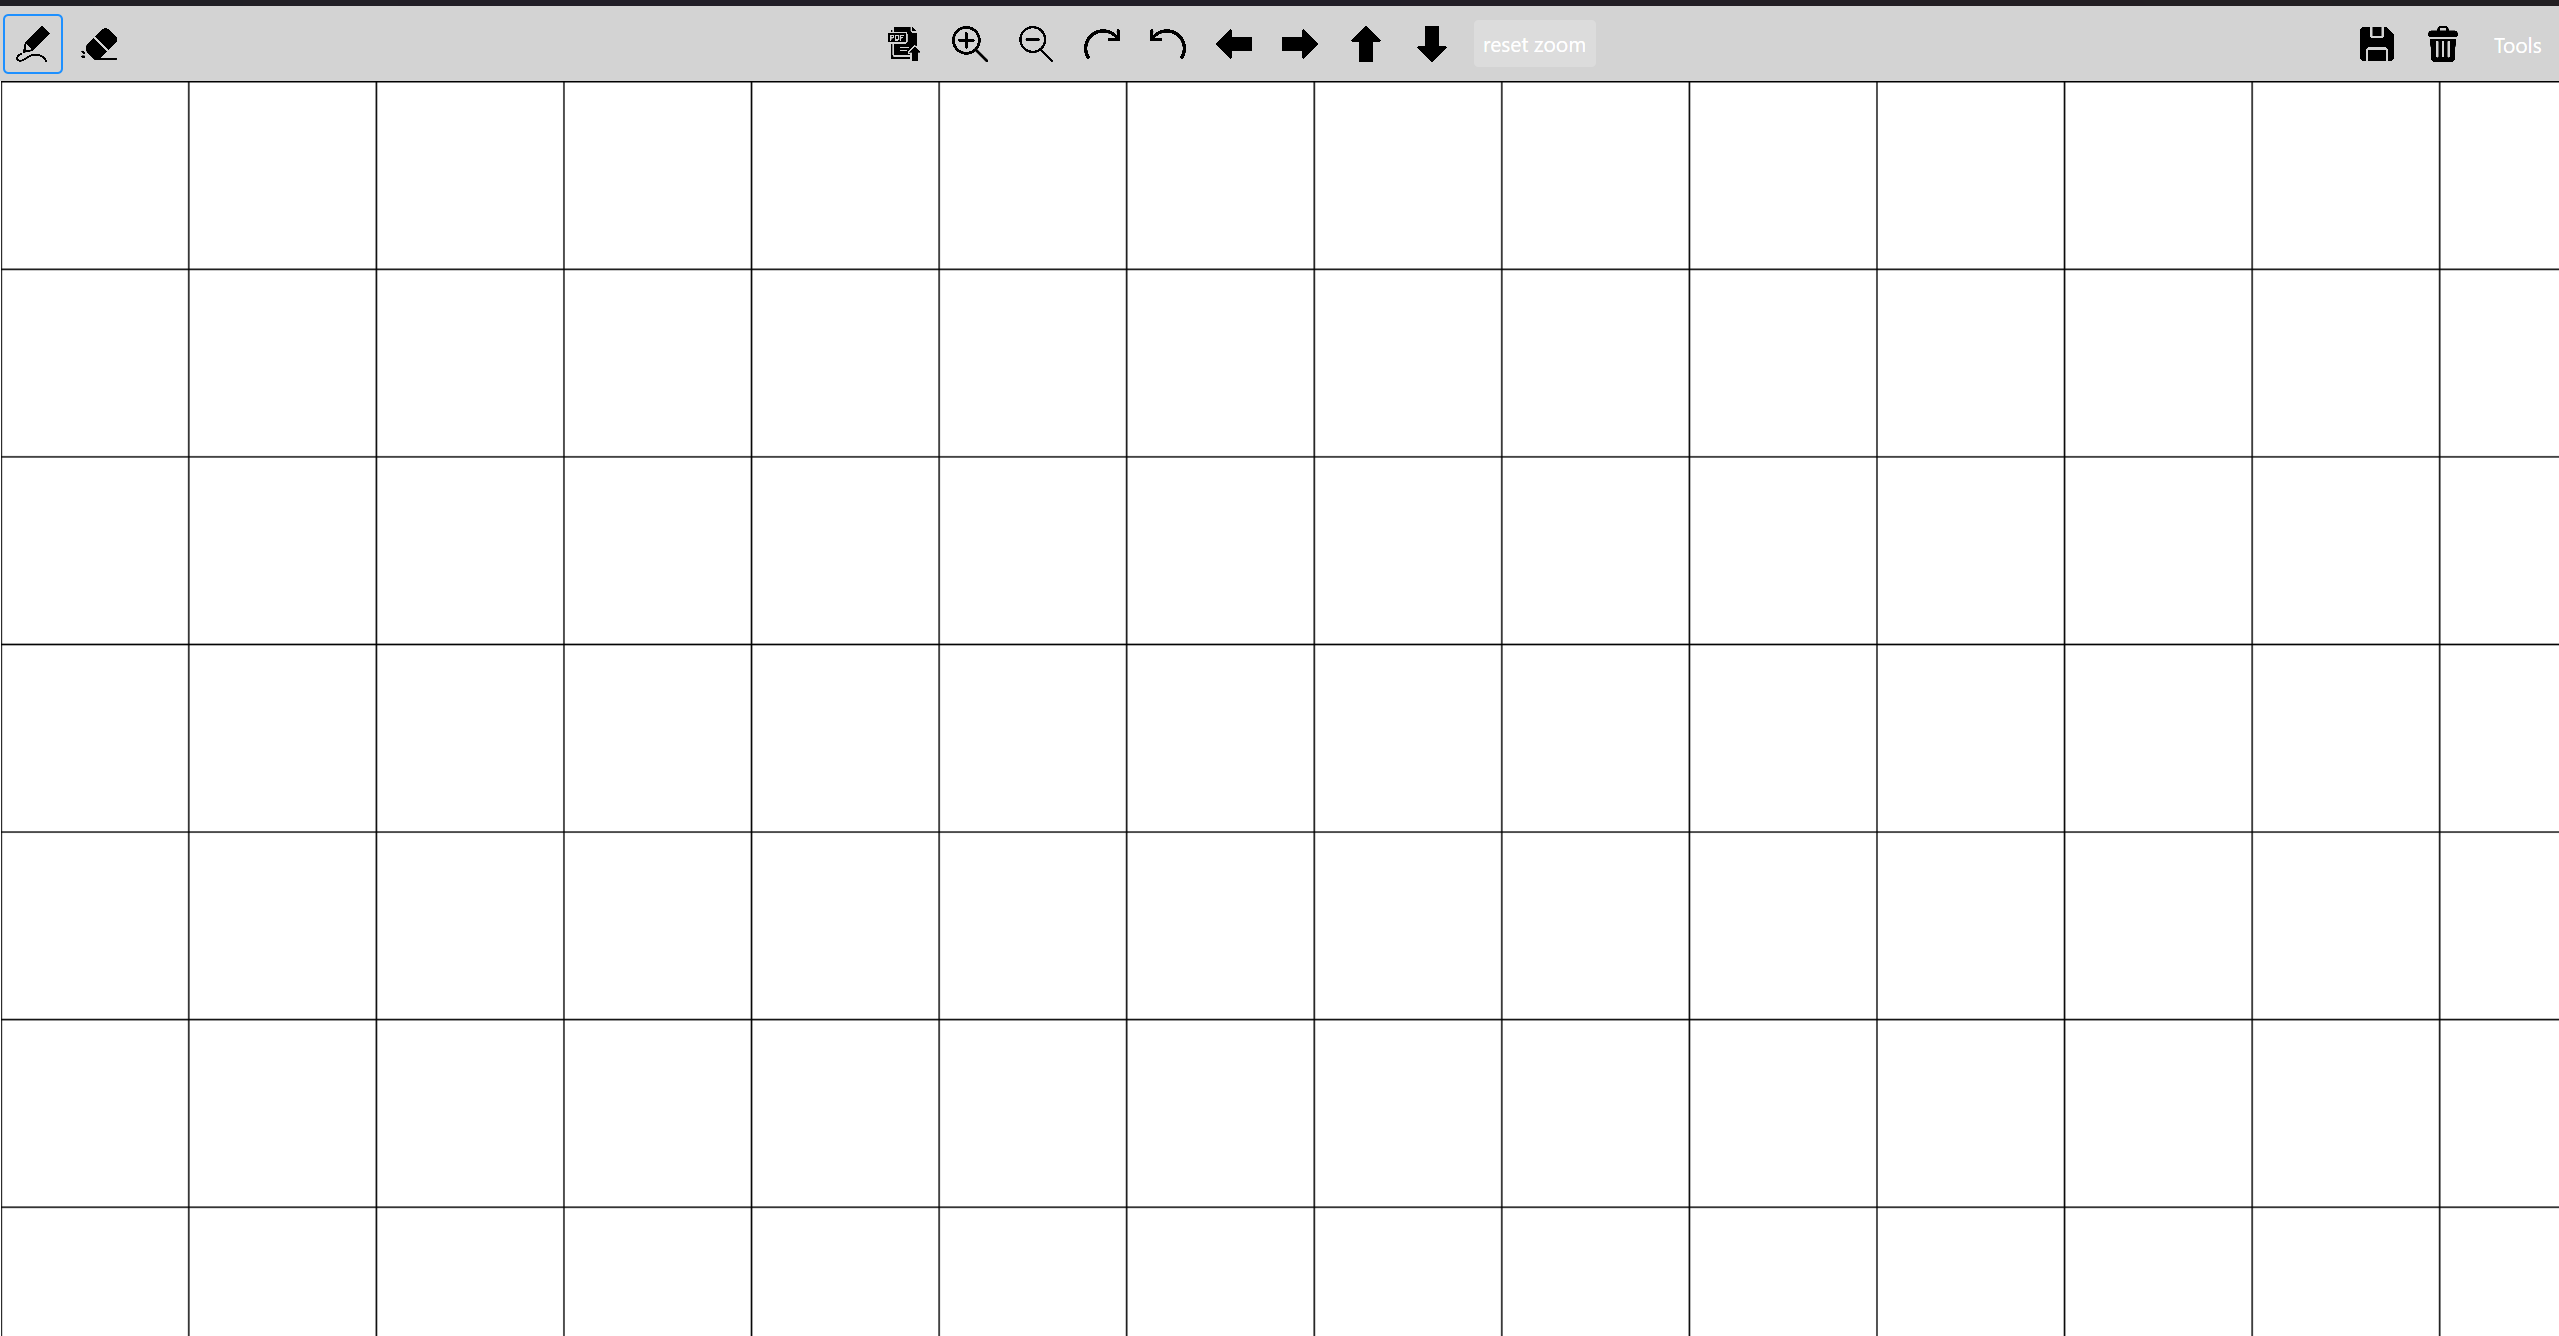
\includegraphics[width=0.75\linewidth]{graphics/ui_screenshot.png}
    \caption{UI Screenshot}
    \label{fig:UI_screenshot}
\end{figure}

Die Benutzeroberfläche besteht aus der Zeichenfläche und einer Werkzeugleiste.\\
Die Werkzeugleiste stellt Funktionen wie Farbauswahl, PDF-Import, Zoom und Pan bereit (detaillierte Dokumentation im Anhang). Für die UI wurde hauptsächlich die Avalonia-Library verwendet.

\vspace{0.5em}
\subsubsection{Zeichenfläche}

Die Zeichenfläche basiert auf einer SKWritableBitmap in einem SKCanvas aus der SkiaSharp-Library. Zeicheneingaben mit Maus oder IR-Stift werden über diese Bitmap dargestellt.

\begin{figure}[H]
  \begin{minipage}{0.48\textwidth}
    \centering
    \frame{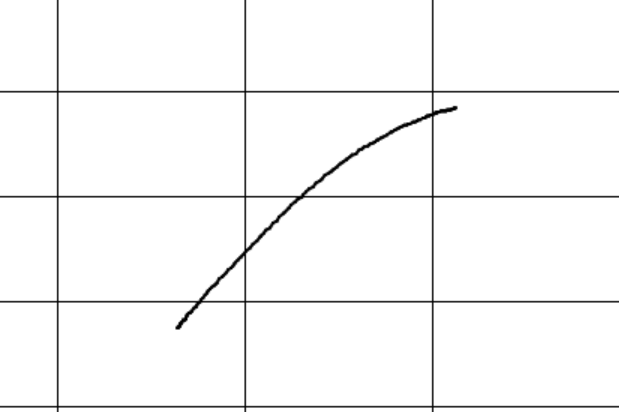
\includegraphics[width=0.9\linewidth]{graphics/bild_strich_in_zeichnungsflaeche.png}}
    \caption{Zeichnungsstrich}
    \label{Fig:Data1}
  \end{minipage}
  \hfill
  \begin{minipage}{0.48\textwidth}
    \centering
    \frame{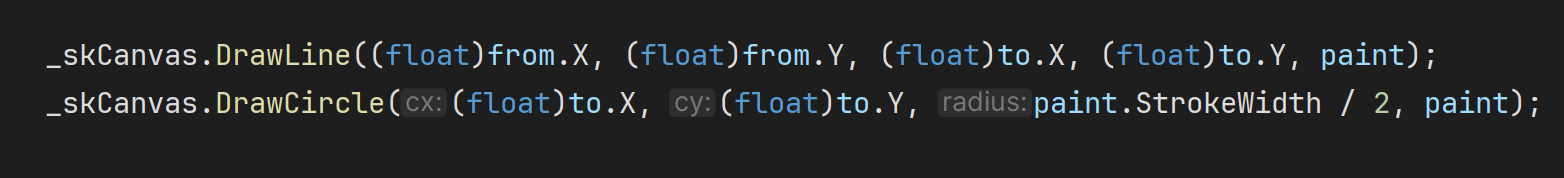
\includegraphics[width=0.9\linewidth]{graphics/code_drawline.png}}
    \caption{Code zur Darstellung eines Striches}
    \label{Fig:Data2}
  \end{minipage}
\end{figure}

\clearpage

Für die Verarbeitung der Stift-Eingaben ist ein Eventhandler zuständig, der auf ein CameraEvent der Klasse InfraredCamera reagiert. Dieser Event informiert die UI-Klasse über erkannte Punkte. Für alle erkannten Punkte in der Liste wird folgende Verarbeitungspipeline durchlaufen:

\begin{figure}[H]
    \centering
    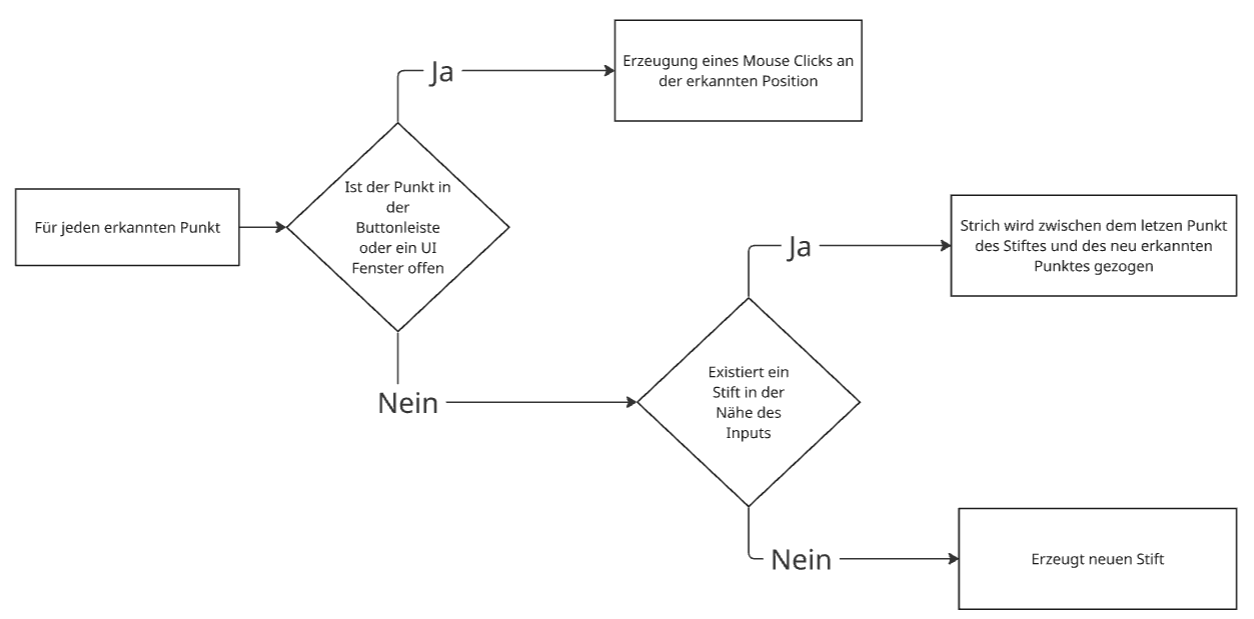
\includegraphics[width=\linewidth]{schema_ablauf_punktdetektion_uiklasse.png}
    \caption{Ablaufschema für die Verarbeitung der erkannten Punkte}
    \label{fig:enter-label}
\end{figure}

Zuerst wird geprüft, ob sich der Punkt im Bereich der Werkzeugleiste befindet. Ist dies der Fall, oder ist durch die Leiste ein Fenster geöffnet, wird der Punkt in einen Mausklick im entsprechenden Screen-Space umgewandelt. So können plattformunabhängig auch systemeigene Dialoge wie etwa Dateiauswahlen bedient werden.
Handelt es sich nicht um einen Steuerungsinput, wird der Punkt als Zeichenbefehl interpretiert. Zur Darstellung einer Linie werden jeweils der aktuelle sowie der letzte Punkt eines Stifts benötigt. Das Tracking erfolgt über eine Liste aller aktiven Stifte, wobei für jeden der letzte Punkt und ein Zeitstempel gespeichert werden. Neue Punkte werden dem wahrscheinlichsten existierenden Stift zugeordnet, basierend auf Distanz und Zeitdifferenz. Falls eine Zuordnung erfolgt, wird eine Linie gezeichnet und die Stiftinformationen aktualisiert.

\clearpage
%\vspace{0.5em}
\subsubsection{Infrarot Stift Erkennung}

Die Erkennung der Stiftspitze erfolgt vollständig innerhalb der InfraredCamera-Klasse. Die Kamera wird über die Intel RealSense SDK angesteuert, die Erkennung erfolgt mit OpenCV.

\begin{figure}[H]
    \centering
    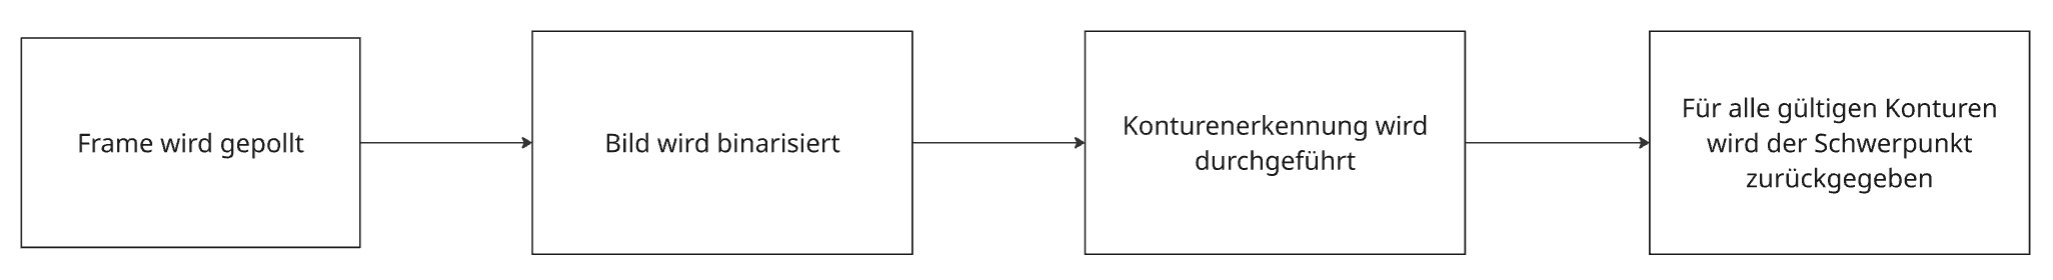
\includegraphics[width=\linewidth]{schema_pen_dedection.png}
    \caption{Ablaufsschema der Stift erkennung}
    \label{fig:enter-label}
\end{figure}

Zunächst werden Bilder der IR-Kamera gepollt:

\begin{figure}[H]
    \begin{minipage}{0.48\textwidth}
    \centering
    \frame{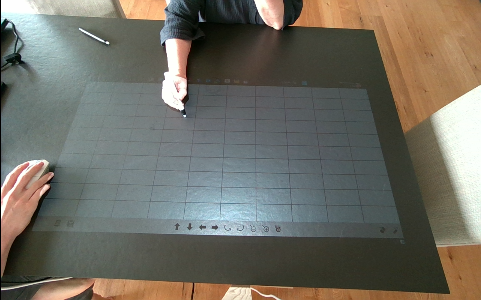
\includegraphics[width=0.9\linewidth]{rgb.png}}
    \caption{Sicht der RGB Kamera}
    \label{Fig:Data1}
  \end{minipage}
  \hfill
  \begin{minipage}{0.48\textwidth}
    \centering
    \frame{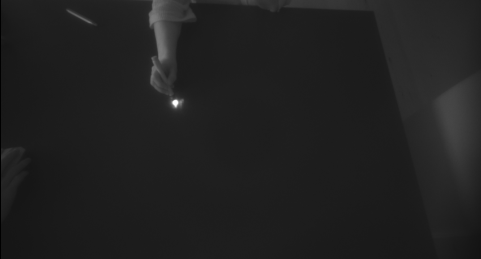
\includegraphics[width=\linewidth]{ir.png}}
    \caption{Sicht der IR Kamera}
    \label{Fig:Data2}
  \end{minipage}
\end{figure}

Diese Bilder werden mittels einfacher Threshold-Binarisierung segmentiert:

\begin{figure}[H]
    \begin{minipage}{0.48\textwidth}
    \centering
    \frame{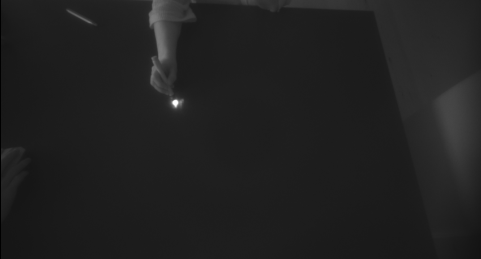
\includegraphics[width=0.9\linewidth]{ir.png}}
    \caption{Sicht der IR Kamera}
    \label{Fig:Data1}
  \end{minipage}
  \hfill
  \begin{minipage}{0.48\textwidth}
    \centering
    \frame{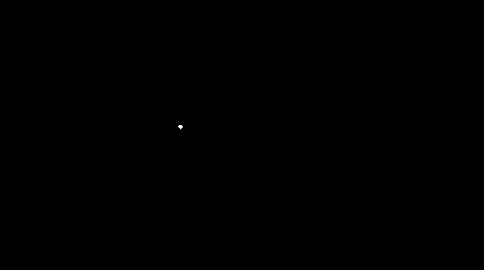
\includegraphics[width=0.9\linewidth]{graphics/binarisiert.png}}
    \caption{Segmentiertes Bild}
    \label{Fig:binarisiert}
  \end{minipage}
\end{figure}

In den segmentierten Bildern werden mit OpenCV die Konturen erkannt. Der Schwerpunkt jedes Blobs in dem segmentierten Bild (Abbildung \ref{Fig:binarisiert}) wird über das zentrale Moment berechnet und als Stiftspitze interpretiert.

\[
x = \frac{M_{10}}{M_{00}}, \quad y = \frac{M_{01}}{M_{00}}
\]
\clearpage

Der erkannte Bildpunkt wird anschliessend per Homographie in den Screenspace übersetzt und zur Liste der gültigen Eingabepunkte hinzugefügt. Die Homographie-Matrix wird ebenfalls mit OpenCV berechnet:

\begin{figure}[H]
    \centering
    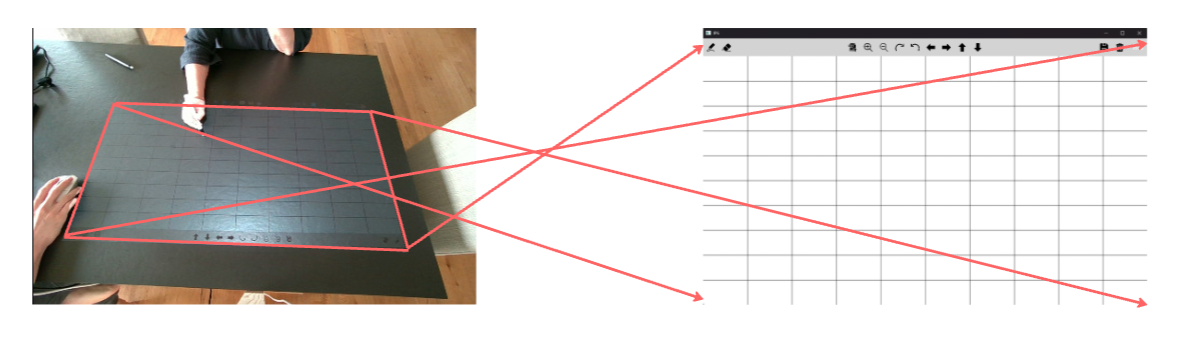
\includegraphics[width=0.9\linewidth]{graphics/homography_graphic.png}
    \caption{Verbildlichung der Homography}
    \label{fig:enter-label}
\end{figure}

\vspace{0.5em}
\subsubsection{Kalibration}

Für die Kalibration werden nacheinander fünf Punkte auf der Zeichenfläche angezeigt:

\begin{figure}[H]
    \centering
    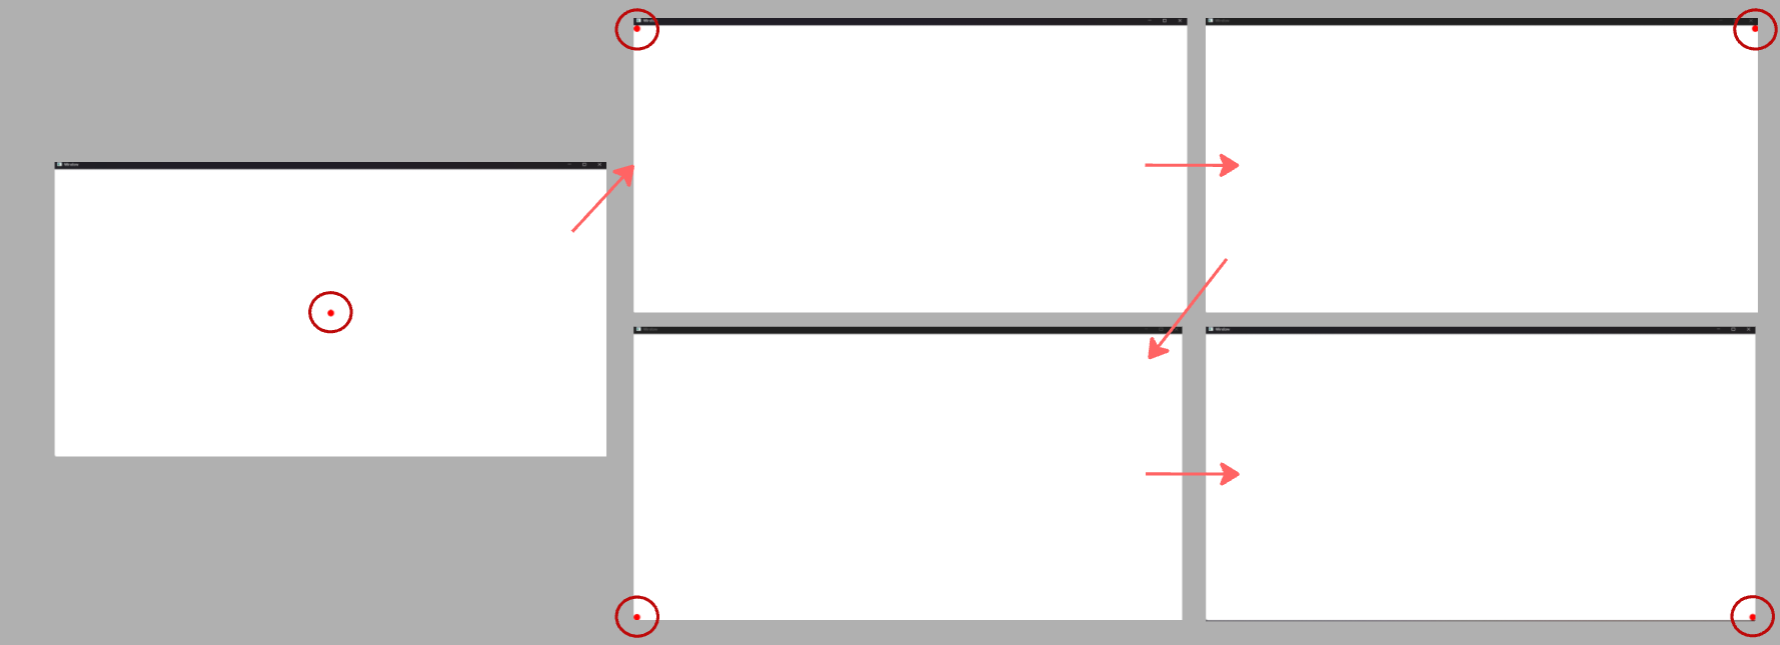
\includegraphics[width=0.9\linewidth]{graphics/ablauf_kalibration.png}
    \caption{Kalibrationsablauf}
    \label{fig:placeholder}
\end{figure}

Bei jedem dieser Punkte wird auf ein CameraEvent gewartet. Der jeweils zuerst erkannte Punkt im Kamerabild wird als entsprechender Kalibrationspunkt im Kameraraum gespeichert.

Diese Punkte im Kamerakoordinatensystem werden anschliessend zusammen mit den bekannten Referenzpunkten im Screen-Space an OpenCV übergeben, um die Homographie-Matrix zu berechnen. Nach erfolgreicher Berechnung der Homographie-Matrix ist die Kalibration abgeschlossen und das Kalibrationsfenster wird automatisch geschlossen.


\section{Auswertung}

Dieses Kapitel präsentiert die Ergebnisse der Evaluation der entwickelten Anwendung im Hinblick auf die in Kapitel \ref{einleitung} formulierten Forschungsfragen.  
Die Auswertung verfolgt das Ziel, die Gebrauchstauglichkeit (Usability), Verständlichkeit sowie die Eignung der Lösung für kollaborative Planungssituationen zu überprüfen.  
Dazu wurden sowohl quantitative Methoden in Form der standardisierten \textit{System Usability Scale} (SUS) als auch qualitative Verfahren wie Beobachtungen, Freitextfeedback und ein praxisnaher Feldtest eingesetzt.  
Diese methodische Kombination ermöglicht es, einerseits messbare, vergleichbare Kennzahlen zu erheben und andererseits detaillierte Einblicke in die Nutzererfahrung und potenzielle Verbesserungspotenziale zu gewinnen.



\subsection{Zielsetzung der Auswertung}

Die Evaluation der entwickelten Anwendung verfolgt das Ziel, ihre Gebrauchstauglichkeit, Verständlichkeit und Eignung für kollaborative Nutzung zu untersuchen. Dabei stehen insbesondere die drei formulierten Forschungsfragen im Fokus:
\begin{itemize}
    \item Wie intuitiv ist die Nutzung für Laien?
    \item Wie verständlich und zugänglich ist die Oberfläche trotz Funktionsvielfalt?
    \item Wie wird die Lösung in realen Anwendungsszenarien wahrgenommen?
\end{itemize}

\subsection{Durchführung und Methodik}

Die Evaluation erfolgte in Form von nutzerzentrierten Usability-Tests mit Teilnehmenden aus der relevanten Zielgruppe. Die Testpersonen bearbeiteten ein Szenario mit mehreren Aufgaben zur Raumgestaltung mithilfe des Infrarotstifts.


Der Ablauf umfasste:
\begin{itemize}
    \item eine kurze Einführung in das System,
    \item die eigenständige Nutzung der Anwendung,
    \item die Beantwortung der System Usability Scale (SUS),
    \item eine Freitext-Rückmeldung sowie
    \item eine passive Beobachtung durch das Projektteam.
\end{itemize}

Zusätzlich wurden Feldtests mit dem Kunden (SCDH) durchgeführt. Dabei wurde das System in realistischen Anwendungsszenarien erprobt und im Anschluss strukturierte Interviews durchgeführt.

\begin{figure}[H]
    \begin{minipage}{0.48\textwidth}
    \centering
    \frame{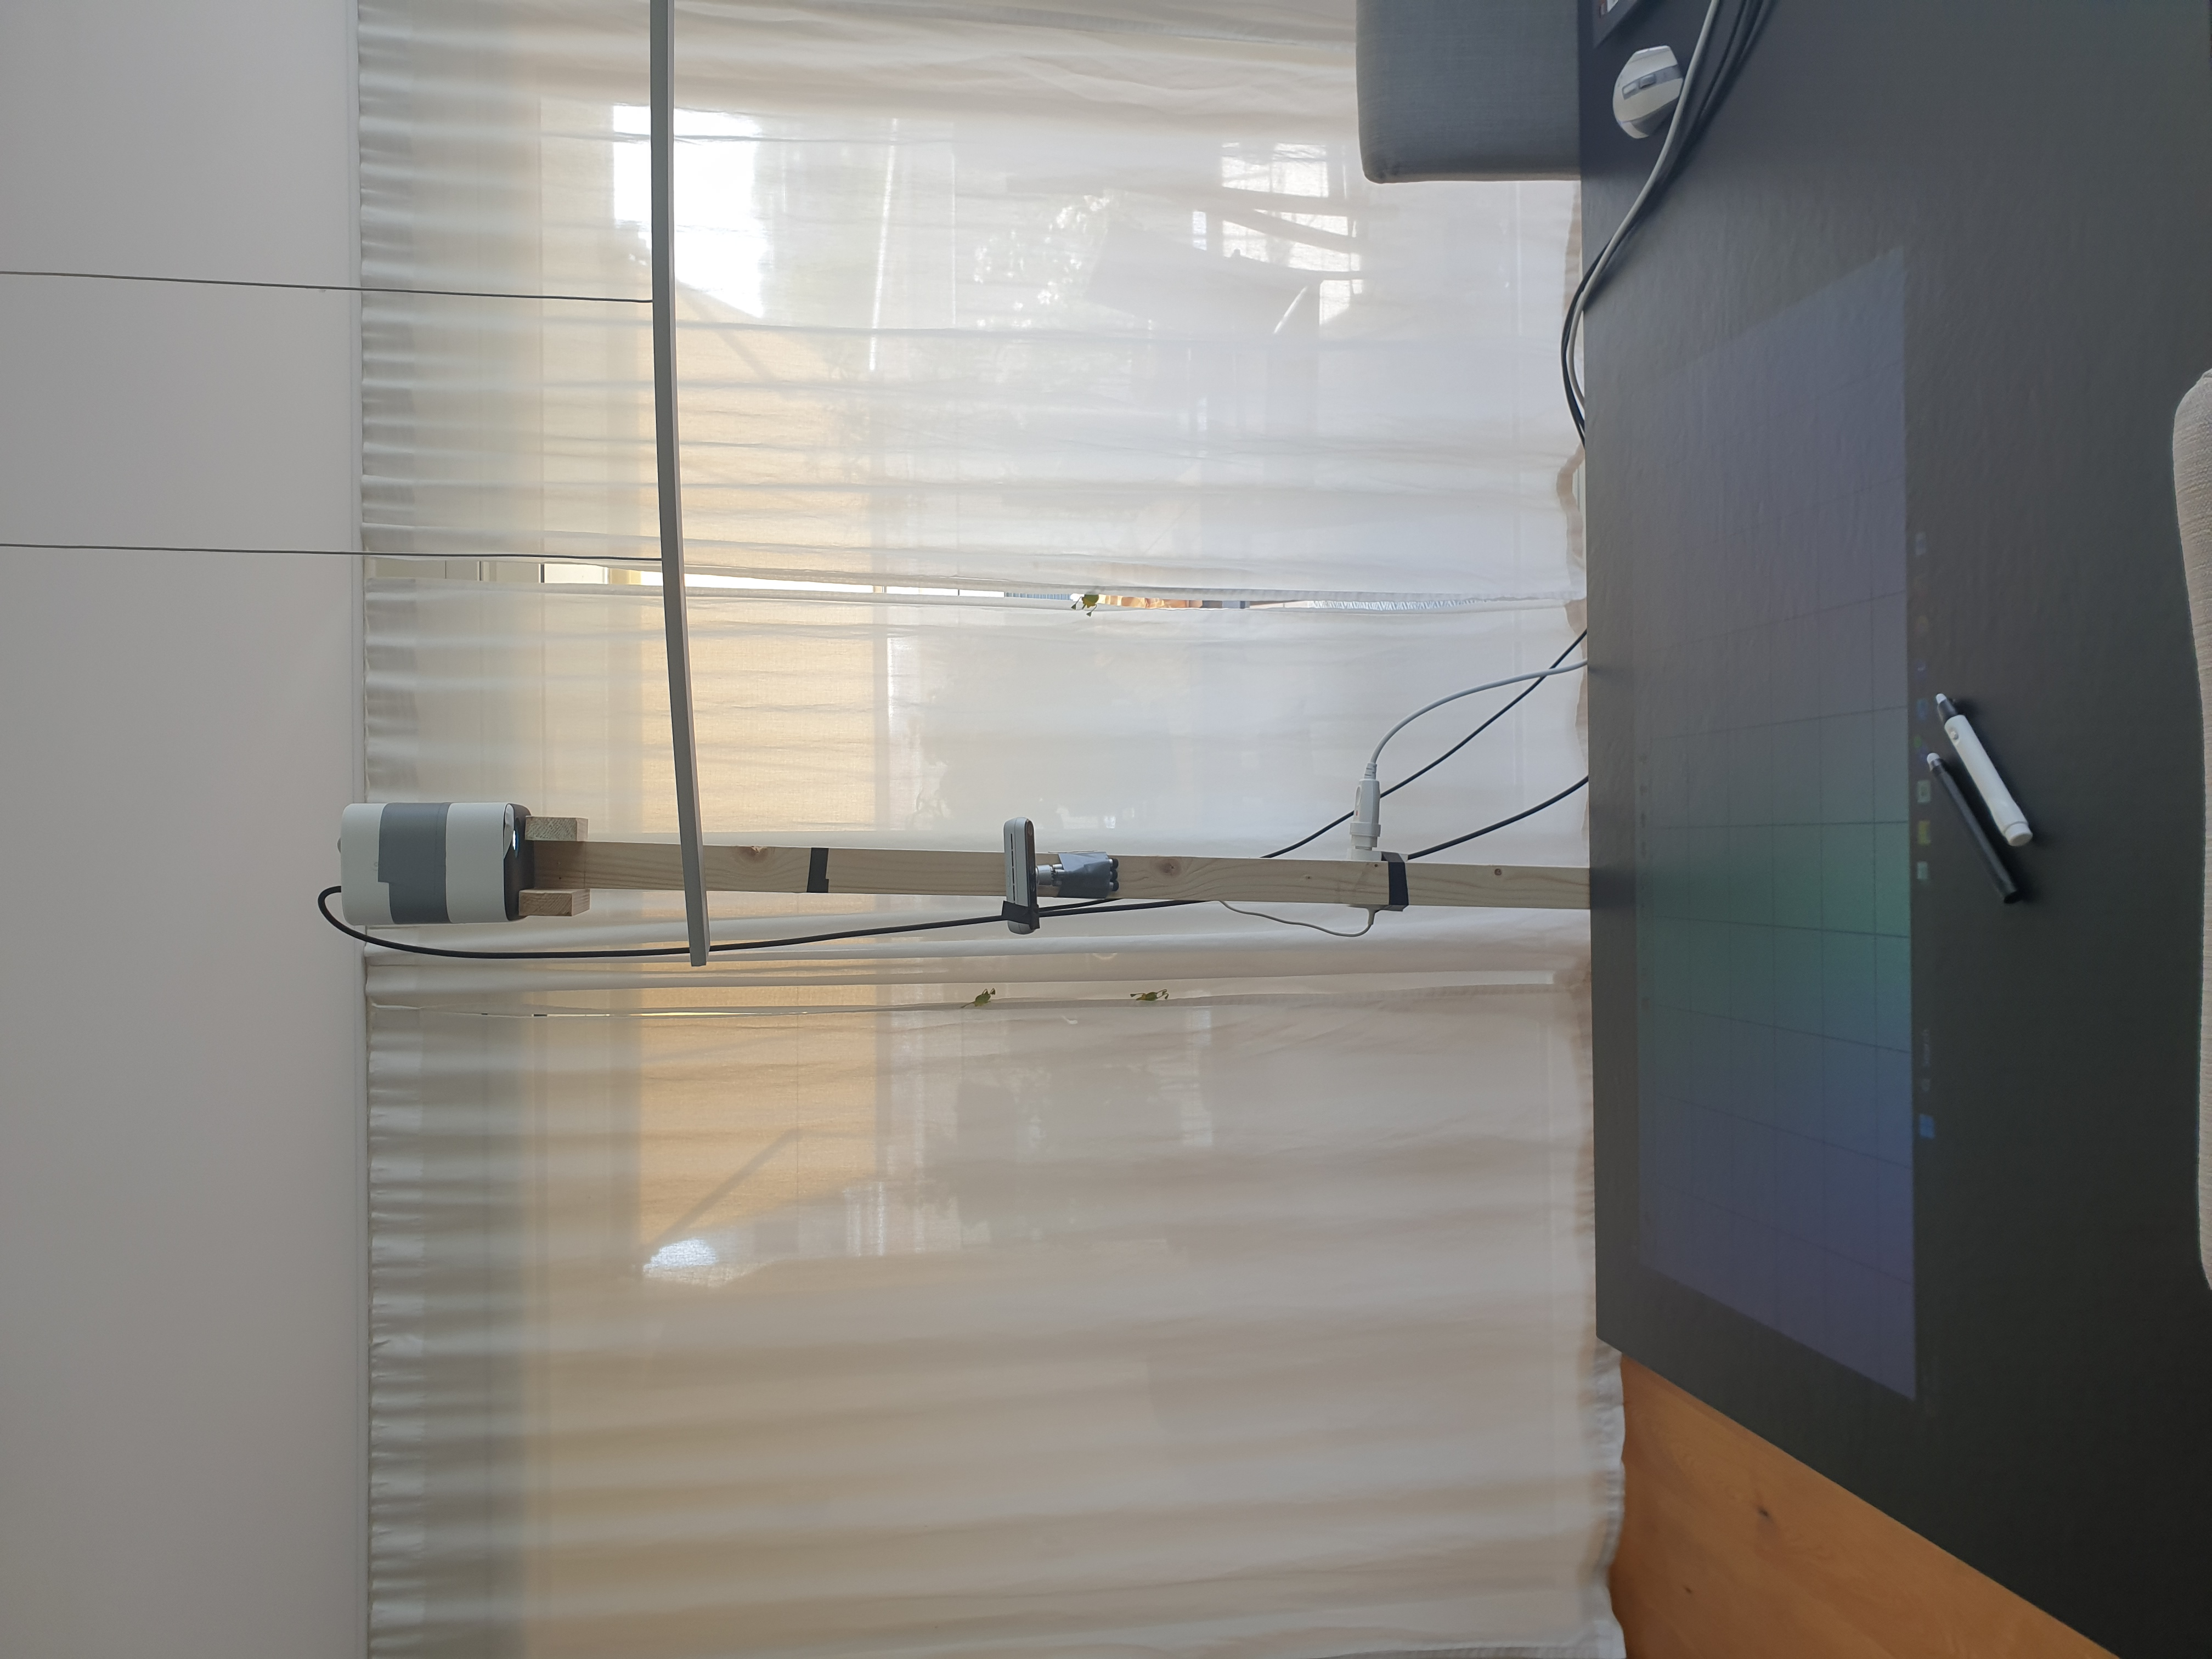
\includegraphics[width=0.7\linewidth, angle=-90]{graphics/sus_setup_1.jpg}}
    \caption{Testaufbau mit Projektion und IR-Stift (SUS)}
    \label{Fig:Data1}
  \end{minipage}
  \hfill
  \begin{minipage}{0.48\textwidth}
    \centering
    \frame{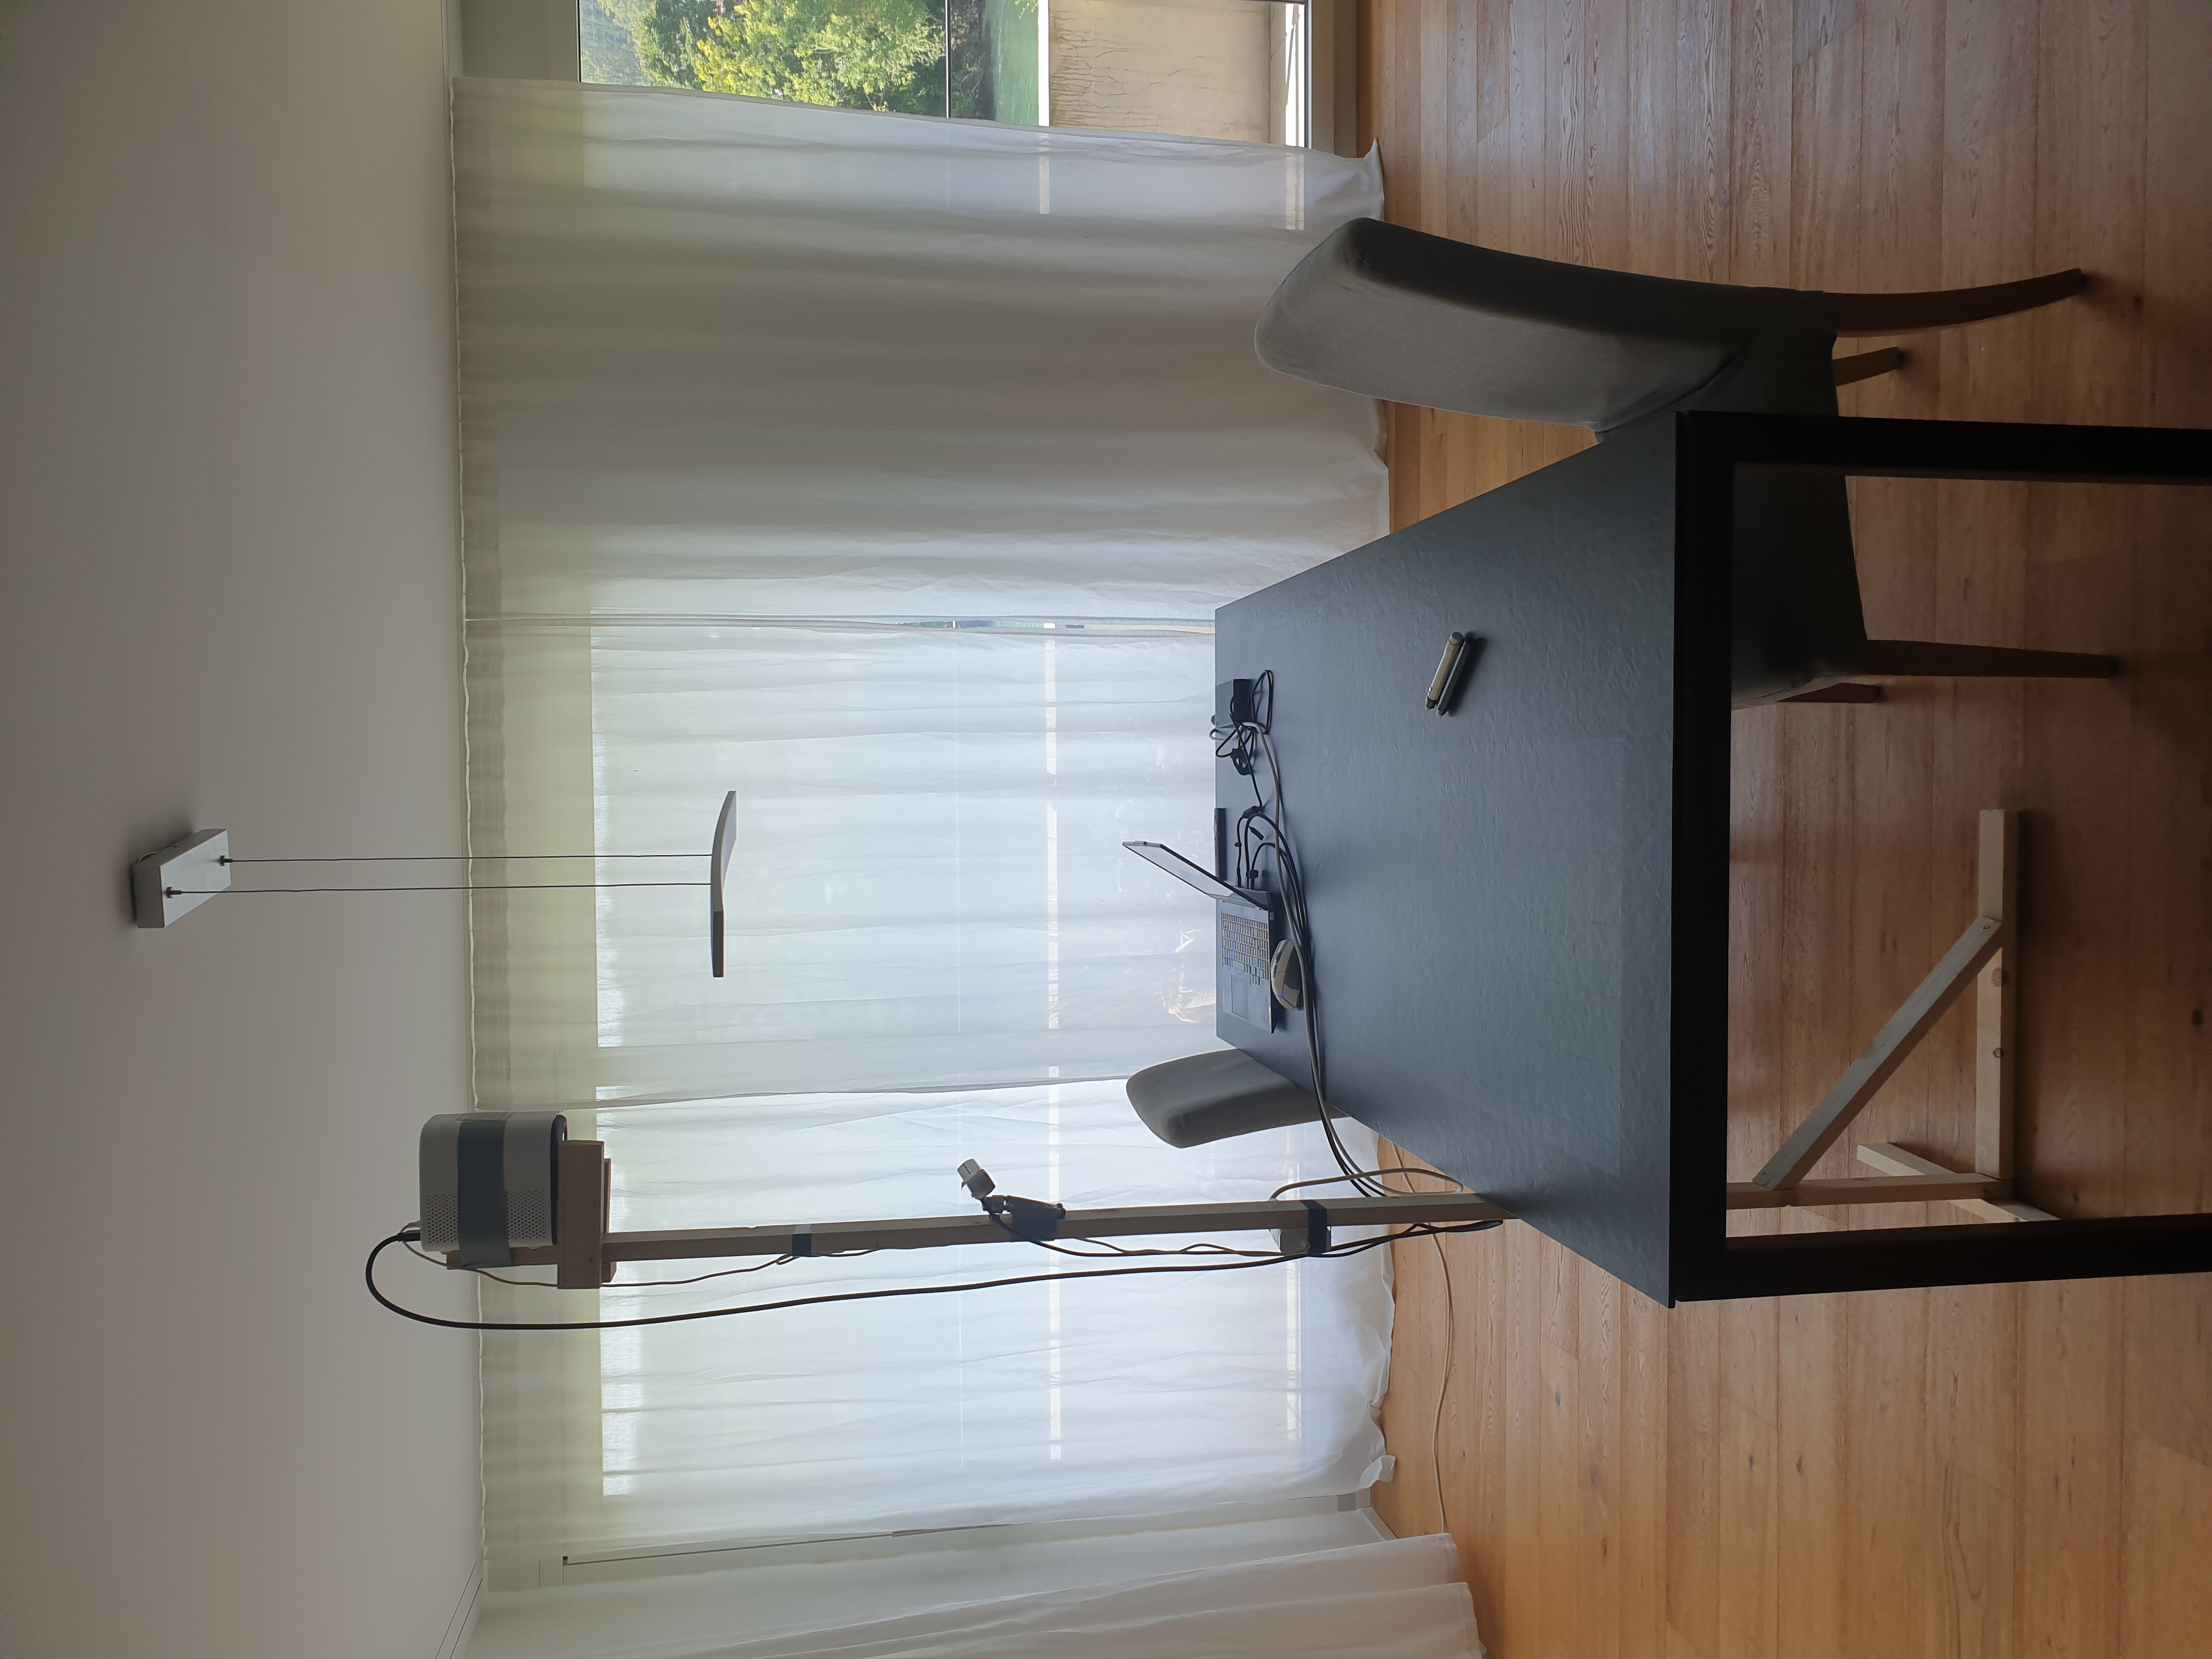
\includegraphics[width=0.7\linewidth, angle=-90]{graphics/sus_setup_2.jpg}}
    \caption{Gesamtansicht der Testumgebung (SUS)}
    \label{Fig:Data2}
  \end{minipage}
\end{figure}


\subsection{SUS-Auswertung}

Zur Bewertung der Gebrauchstauglichkeit wurde die etablierte Methode des \textit{System Usability Scale} (SUS) verwendet. Der SUS ist ein standardisiertes Umfrageinstrument, das aus zehn Aussagen besteht, die von den Teilnehmenden auf einer fünfstufigen Likert-Skala (von „stimme überhaupt nicht zu“ bis „stimme voll und ganz zu“) bewertet werden. Der SUS ist bewusst allgemein gehalten, um auf unterschiedlichste digitale Systeme angewendet werden zu können. Er erfasst sowohl die wahrgenommene Einfachheit als auch die Effizienz der Nutzung und erlaubt einen Vergleich mit anderen Systemen anhand eines normierten Scores. Ein Mittelwert von 68 gilt dabei als durchschnittliche Usability. Im Rahmen des Tests mit vier Teilnehmenden wurde der SUS nach Abschluss der praktischen Erprobung der Anwendung ausgefüllt. Die Ergebnisse wurden anschliessend mithilfe einer standardisierten Template-Berechnung ausgewertet, bei der jedem Item ein Punktewert zugeordnet und auf eine Skala von 0 bis 100 normiert wird. Diese Vorgehensweise bietet eine einfache und zugleich wissenschaftlich etablierte Möglichkeit, die wahrgenommene Benutzerfreundlichkeit zu quantifizieren. Sie eignet sich insbesondere für kleinere Testgruppen und liefert dennoch verlässliche Aussagen über die grundsätzliche Akzeptanz und Bedienbarkeit eines Systems.\\  \cite{brooke1986sus} \cite{uiuxtrendSUS}

Die Bewertungen ergaben folgende Scores:
\begin{itemize}
    \item \textbf{Person 1:} 67.5 Punkte
    \item \textbf{Person 2:} 85.0 Punkte
    \item \textbf{Person 3:} 75.0 Punkte
    \item \textbf{Person 4:} 70.0 Punkte
    \item \textbf{Person 5:} 87.5 Punkte
    \item \textbf{Person 6:} 85.0 Punkte
\end{itemize}

Der Mittelwert liegt bei \textbf{78.33 Punkten}. Dies weist auf eine insgesamt gute bis sehr gute Gebrauchstauglichkeit der Anwendung hin. Abbildung~\ref{fig:sus_scores_updated_v2} visualisiert die Ergebnisse im Vergleich zum Standardbenchmark.

\begin{figure}[H]
    \centering
    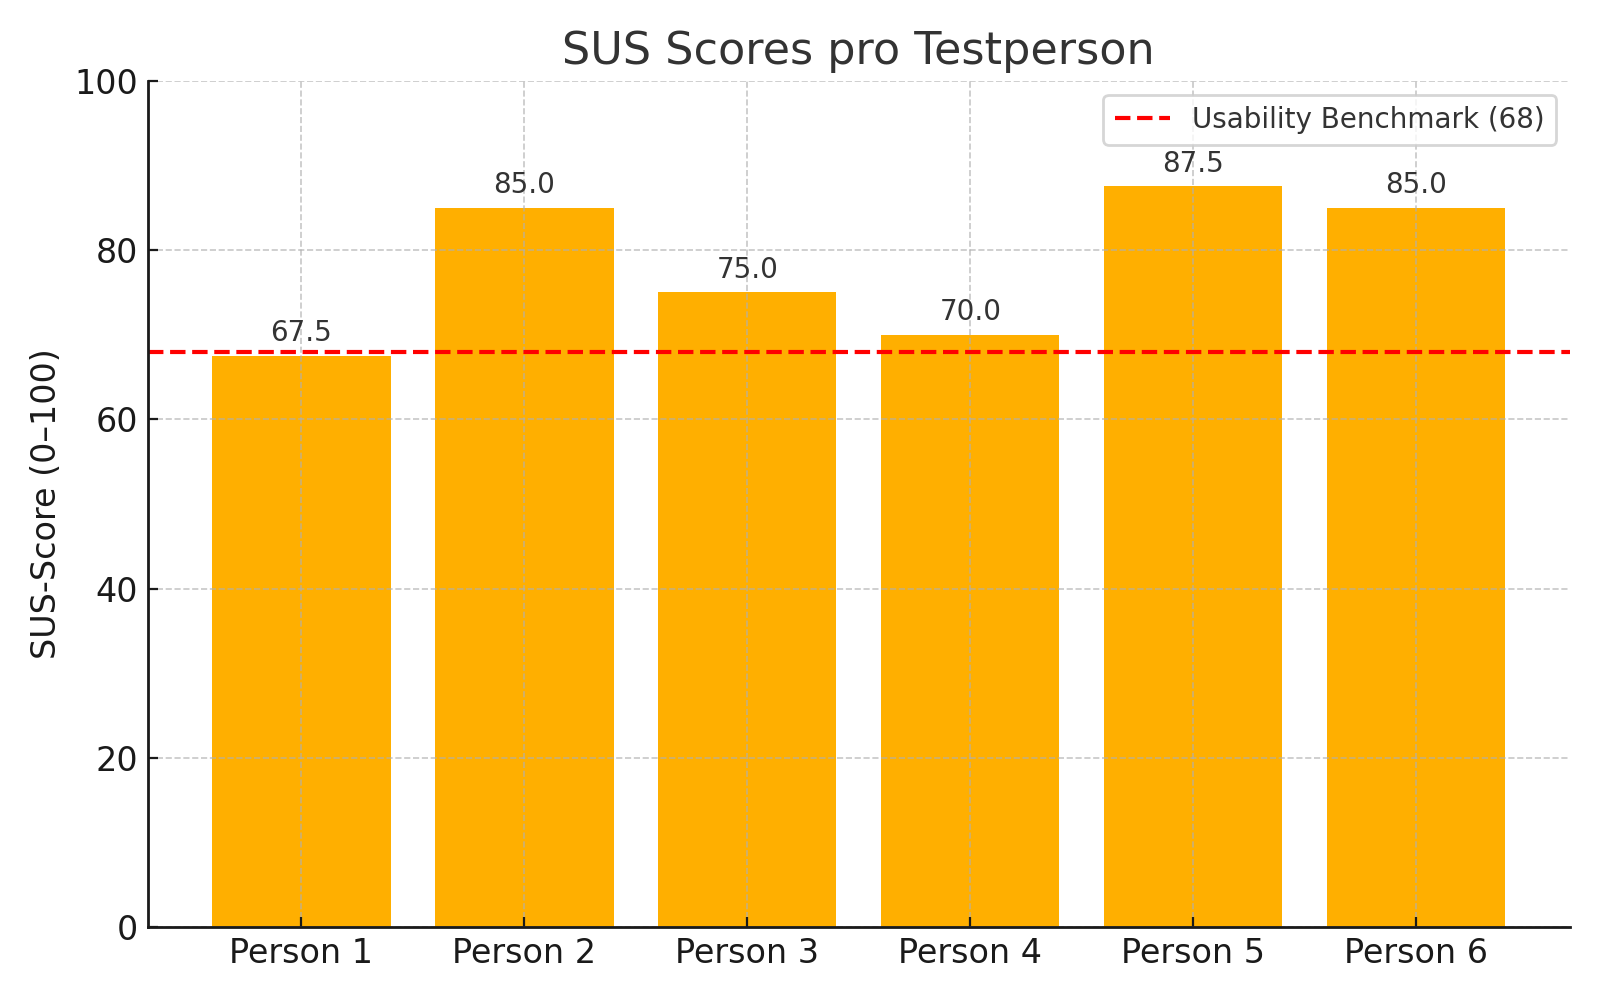
\includegraphics[width=0.65\textwidth]{graphics/sus_scores_plot.png}
    \caption{SUS-Bewertung aller Testpersonen im Vergleich zum Benchmark (68 Punkte)}
    \label{fig:sus_scores_updated_v2}
\end{figure}

\clearpage

\subsection{Qualitatives Feedback und Beobachtungen}

Neben der quantitativen Bewertung wurde zusätzlich qualitatives Feedback in Form von offenen Fragen und Beobachtungen erhoben. Dieses qualitative Feedback ermöglicht eine vertiefte Analyse und liefert detaillierte Einblicke in die Stärken und Schwächen der Anwendung. Dadurch können nicht nur allgemeine Tendenzen, sondern auch spezifische Verbesserungspotenziale identifiziert werden, die in der quantitativen Auswertung möglicherweise nicht erkennbar sind.


\textbf{Positiv bewertet wurden:}
\begin{itemize}
    \item Das grundlegende Konzept wurde mehrfach positiv beurteilt. Insbesondere das freie Zeichnen auf einer beliebigen Zeichenfläche kam bei fast allen Testpersonen sehr gut an.
    \item Die einfache und intuitive Bedienung wurde durchgehend als positiv empfunden.
\end{itemize}

\textbf{Herausforderungen und Verbesserungspotenziale:}
\begin{itemize}
    \item Es herrschte Unsicherheit bezüglich der Bedeutung einzelner Icons. So wurde beispielsweise das Rotations-Icon von mehreren Testpersonen fälschlicherweise als „Undo“-Button interpretiert.
    \item Bei einigen Tests traten noch Bugs sowie Präzisionsprobleme auf, welche negativ auffielen.
    \item Die Radierfunktion erhielt gemischtes Feedback. Einige Nutzer wünschten sich mehr Auswahlmöglichkeiten bezüglich der Funktionsweise. Insbesondere wurde kritisiert, dass der Hintergrund mitgelöscht wird. Dies wurde von einigen Personen negativ bewertet, während andere die Funktion grundsätzlich akzeptierten, jedoch einen separaten Modus forderten, um Striche oder Bereiche zu löschen, ohne den Hintergrund zu beeinträchtigen.
\end{itemize}



Grundsätzlich wurden vor allem fehlende Funktionen sowie Funktionen mit unzureichendem Umfang negativ bewertet, während die Qualität und Verständlichkeit insgesamt als gut eingeschätzt wurden. Das qualitative Feedback und die Beobachtungen erwiesen sich dabei als besonders wertvoller Input. So wurde beispielsweise bereits bei der ersten Testperson festgestellt, dass das ursprüngliche Konzept für ein Setup mit einer Kamera im 90°-Winkel zur Zeichenfläche nicht optimal ist. Dieses Problem konnte daraufhin unmittelbar behoben werden, sodass es bei allen nachfolgenden Tests nicht mehr auftrat.
\clearpage

\subsection{Feldtest mit Kundeninterview}

Um das Verhalten des Systems in einer möglichst realitätsnahen Umgebung zu prüfen, wurde ein Feldtest direkt beim SCDH in Nidau durchgeführt. 
Dabei wurde das System vor Ort installiert und im Rahmen einer Demonstration für den SCDH ein simulierter Workshopablauf durchgespielt. 
Anschliessend wurde ein Interview mit David Wollschlegel geführt, um seine Einschätzung zum System einzuholen. 
Dabei wurden verschiedene Punkte zum System, zu den Integrationsmöglichkeiten sowie zu Verbesserungs- und Erweiterungspotenzialen erörtert. 
Insgesamt zeigte sich David Wollschlegel sehr zufrieden mit dem Endstand des Projekts.


\begin{figure}[H]
    \centering
    \includegraphics[width=0.65\linewidth]{graphics/übersicht_feldtest.JPG}
    \caption{Setup beim Feldtest im SCDH}
    \label{fig:placeholder}
\end{figure}

\textbf{Positive Punkte:}
\begin{itemize}
    \item Das System erfüllt grundsätzlich die gestellten Anforderungen.
    \item Es fügt sich bereits gut in die bestehenden Arbeitsprozesse des SCDH ein.
    \item Insgesamt weist es ein vielversprechendes Potenzial auf und bietet einen klaren Mehrwert gegenüber bestehenden Methoden und Möglichkeiten.
\end{itemize}

\textbf{Negative Punkte:}
\begin{itemize}
    \item Ein leichter Offset wurde als geringfügig störend wahrgenommen, jedoch nicht als gravierend bewertet.
\end{itemize}

\textbf{Feedback zur Zukunft:}
\begin{itemize}
    \item Mögliche Hürden bei der Einführung in ein produktives Umfeld am SCDH liegen nicht im System selbst, sondern in der Beschaffung, dem Setup vor Ort sowie der Integration in die bestehende Softwarelandschaft des SCDH.
    \item Das System bietet dem SCDH die Möglichkeit, neue Angebote zu entwickeln.
    \item Es wurden verschiedene Feature-Wünsche und Ideen besprochen, beispielsweise ein Objektkatalog, Cloud- und Remote-Funktionen sowie weitere Features und \emph{Quality-of-Life}-Verbesserungen.
\end{itemize}


\begin{figure}[H]
    \centering
    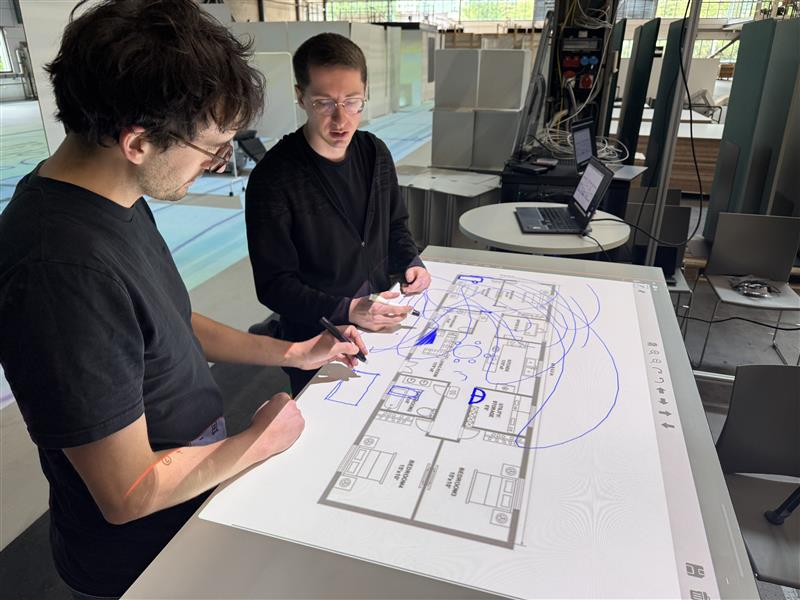
\includegraphics[width=0.65\textwidth]{graphics/feldtest.JPG}
    \caption{Feldtest am SCDH mit dem Kunden}
    \label{fig:feldtest}
\end{figure}

\subsection{Fazit}

Die Tests zeigten, dass die Anwendung sehr gut angenommen wird. Der durchschnittliche SUS-Wert liegt mit 78.33 Punkten deutlich über dem branchenüblichen Schwellenwert von 68 Punkten und bestätigt damit eine hohe Gebrauchstauglichkeit.  
Da die Bewertung nach der anerkannten \textit{System Usability Scale} (SUS) erfolgte, sind die Ergebnisse gut mit anderen Studien und Systemen vergleichbar und unterstreichen die methodische Validität der Erhebung.  

Neben den positiven quantitativen Ergebnissen lieferten auch die qualitativen Rückmeldungen wertvolle Hinweise für mögliche Optimierungen. Der durchgeführte Feldtest mit dem Kunden bestätigte die Praxistauglichkeit der Lösung und identifizierte zentrale Verbesserungspotenziale wie eine optimierte Kalibrierung, zusätzliche Funktionen wie Undo/Redo sowie erweiterte Integrationsmöglichkeiten.  

Insgesamt steht fest, dass die entwickelte Lösung sowohl in ihrer aktuellen Form produktiv eingesetzt werden kann als auch eine solide Basis für zukünftige Erweiterungen bietet. Der erzielte Entwicklungsstand erfüllt die gesteckten Projektziele vollständig und belegt das Potenzial des Systems für den langfristigen Einsatz in unterschiedlichen Anwendungskontexten.



\section{Diskussion}

In diesem Kapitel werden die Ergebnisse und Beobachtungen im Rahmen des Projekts kritisch reflektiert. Dabei stehen sowohl die Einordnung der Lösung in den Anwendungskontext als auch ihre Stärken, Schwächen und offene Fragen im Vordergrund.

\subsection{Erfüllung der Projektziele}

Die entwickelte Anwendung erfüllt die grundlegenden Anforderungen, die in der Aufgabenstellung und in den Workshops definiert wurden.  
Nutzer:innen können mit dem IR-Stift intuitiv auf einer Projektionsfläche zeichnen, Inhalte in Echtzeit anpassen und gemeinsam an Raumkonzepten arbeiten.  
Besonders positiv hervorzuheben ist die niedrige Einstiegshürde für Laien sowie die plattformübergreifende Architektur.

Die im Rahmen der Usability-Tests erreichten Ergebnisse bestätigen den Erfolg der Umsetzung: Mit einem durchschnittlichen SUS-Wert von 78.33 Punkten liegt die Anwendung deutlich über dem branchenüblichen Schwellenwert von 68 Punkten und weist somit eine hohe Gebrauchstauglichkeit auf.  
Auch der durchgeführte Feldtest mit dem Kunden hat die Praxistauglichkeit der Lösung unter realistischen Bedingungen bestätigt und wertvolle Hinweise zur Weiterentwicklung geliefert.  
Diese Kombination aus hoher Benutzerfreundlichkeit und positiver Rückmeldung aus der realen Anwendung belegt, dass die gesteckten Projektziele nicht nur erfüllt, sondern in wesentlichen Aspekten übertroffen wurden.


\subsection{Einordnung in den Anwendungskontext}

Der Einsatz im Workshop-Kontext am SCDH hat sich als besonders sinnvoll erwiesen.  
Die Lösung adressiert reale Herausforderungen wie Kommunikationsbarrieren, unklare Türrichtungen oder mangelnde Flexibilität bei kurzfristigen Änderungen.  
Durch die direkte Visualisierung auf der 1:1-Projektionsfläche können Anpassungen ohne Zeitverlust umgesetzt und allen Teilnehmenden sofort präsentiert werden.

Ein wesentlicher Vorteil für das SCDH liegt in der hohen Flexibilität des Systems.  
Es lässt sich sowohl mit bestehenden Grundrissplänen als auch auf einer leeren Projektionsfläche einsetzen und unterstützt so unterschiedliche Workshop-Formate von der frühen Konzeptphase bis zur detaillierten Layoutdiskussion.  
Zudem kann das System schnell auf neue Szenarien angepasst werden, ohne dass zusätzliche Schulungen oder technisches Vorwissen erforderlich sind.  

Der Feldtest hat gezeigt, dass diese Flexibilität in der Praxis von grossem Vorteil ist.  
So können Änderungen während des Workshops sofort als Bild exportiert und den Architekt:innen zur weiteren Bearbeitung bereitgestellt werden, ohne den Umweg über einen schriftlichen Bericht gehen zu müssen.  
Diese Eigenschaften ermöglichen es dem SCDH, die Anwendung nicht nur in partizipativen Workshops mit Laien, sondern auch in Projekten mit Architekt:innen, Planungsämtern und weiteren Fachdisziplinen einzusetzen.

\clearpage

\subsection{Reflexion der Forschungsfragen}

Die im Projekt formulierten Forschungsfragen lassen sich rückblickend wie folgt einordnen:

\begin{itemize}
    \item \textbf{Forschungsfrage 1} (Systemgestaltung für kollaborative Planung): konnte klar beantwortet werden. Durch den Einsatz des IR-Stifts, die Echtzeitprojektion und die Möglichkeit der gleichzeitigen Nutzung durch mehrere Personen wurde eine effektive kollaborative Arbeitsweise ermöglicht. Sowohl die Usability-Tests als auch der Feldtest haben bestätigt, dass der Arbeitsfluss deutlich verbessert und Missverständnisse reduziert werden konnten.

    
    \item \textbf{Forschungsfrage 2} (intuitive Benutzeroberfläche für Laien): die Tests zeigen, dass die Stift-Metapher und das visuelle Feedback ohne zusätzliche Schulung verstanden werden. Die hohe durchschnittliche Bewertung von 78.33 Punkten im SUS unterstreicht, dass die Bedienung auch für Erstnutzende zugänglich und leicht verständlich ist. Beobachtungen bei den Tests zeigten, dass selbst Personen ohne technische Erfahrung nach kurzer Einweisung eigenständig arbeiten konnten.
    
    \item \textbf{Forschungsfrage 3} (Usability in realen Szenarien): der Feldtest mit dem Kunden hat gezeigt, dass die Lösung im praktischen Einsatz nicht nur angenommen, sondern aktiv als hilfreiches Werkzeug in Workshops wahrgenommen wird. Besonders die Fähigkeit, flexibel auf neue Anforderungen zu reagieren und Ergebnisse sofort zu visualisieren, wurde positiv hervorgehoben.
\end{itemize}


\subsection{Grenzen der Lösung}

Die Ergebnisse der Usability-Tests haben deutlich gemacht, dass für einen produktiven Einsatz zusätzliche Funktionen erforderlich sind und bestehende Funktionen in ihrer Umsetzung weiter optimiert werden sollten.  
Zwar unterstützt das System die Arbeit mit mehreren Stiften gleichzeitig, jedoch können diese aktuell nicht voneinander unterschieden werden. Dies bedeutet, dass alle Stifte dieselben Einstellungen verwenden.  

Aus technischer Sicht ist das System zudem durch die Verwendung einer einzelnen Kamera limitiert.  
Für eine zuverlässigere Erkennung wäre der Einsatz von mindestens einer weiteren Kamera sinnvoll, um zu verhindern, dass die Handhaltung die Stiftspitze verdeckt und dadurch die Erfassung unterbrochen wird.

\clearpage

\subsection{Offene Fragen und Ausblick}

Einige offene Fragen konnten im Rahmen des Projekts nur teilweise beantwortet werden und bilden Ansatzpunkte für zukünftige Arbeiten.  
Dazu gehört insbesondere die Frage, wie sich die Usability bei mehreren aktiven Nutzer:innen gleichzeitig verhält.  
Hier könnte eine optimierte Eingabeverwaltung helfen, Überschneidungen und unbeabsichtigte Interaktionen zu minimieren.

Aus dem Feldtest gingen zudem konkrete Funktionswünsche hervor:  
Eine Undo/Redo-Funktion, ein integrierter Objektkatalog, erweiterte Exportmöglichkeiten (z. B. PDF-Export oder direkter Versand an Projektbeteiligte) sowie eine präzisere Kalibrierung wurden mehrfach genannt.  
Auch die Möglichkeit zur Unterstützung von Multi-Display-Setups und Remote-Zusammenarbeit könnte den Einsatzbereich erheblich erweitern, etwa für hybride Workshops oder parallele Planungssitzungen.  

Darüber hinaus wäre die Integration zusätzlicher Visualisierungsmöglichkeiten wie farbliche Layer oder Objektschatten ein potenzieller Mehrwert,  
um komplexere Entwürfe übersichtlicher darzustellen.  
Langfristig könnte auch eine Cloud-Anbindung zur Speicherung und Nachverfolgung von Workshop-Ergebnissen sowie eine Tablet-basierte Steuerung  
zur Ergänzung der Projektion implementiert werden.  

Diese Weiterentwicklungen würden nicht nur die Funktionalität und Flexibilität des Systems erhöhen,  
sondern auch seine Attraktivität für weitere Zielgruppen wie Architekturbüros, städtische Planungsämter oder technische Gewerke deutlich steigern.

\section{Schlusswort}

Im Rahmen dieses Projekts wurde eine interaktive Zeichenanwendung entwickelt, die es Laien ermöglicht, auf einer 1:1-Projektionsfläche funktionale Raumkonzepte kollaborativ zu entwerfen und direkt zu erleben.  
Die Lösung wurde bewusst benutzerzentriert konzipiert und in enger Abstimmung mit realen Anwendungsbedürfnissen, insbesondere im Kontext von partizipativen Architektur-Workshops am SCDH, umgesetzt.  

Durch den Einsatz eines Infrarotstifts und einer kamerabasierten Erkennung konnte eine präzise, flexible und kostengünstige Eingabemethode realisiert werden.  
Die entwickelte Software überzeugte sowohl in den Usability-Tests, mit einem durchschnittlichen SUS-Wert von 78.33 Punkten deutlich über dem branchenüblichen Schwellenwert, als auch im Feldtest mit dem Kunden, der die Praxistauglichkeit unter realistischen Bedingungen bestätigte.  

Auch wenn nicht alle Funktionen vollständig ausgereift oder umgesetzt wurden, wie etwa automatische Kalibrierung, Undo/Redo oder eine softwareseitige Mehrbenutzerverwaltung, zeigt das Ergebnis klar das Potenzial für den Praxiseinsatz.  
Die Forschungsfragen wurden weitgehend beantwortet und die Lösung bildet eine solide Grundlage für weiterführende Arbeiten, etwa zur Evaluation unter realen Bedingungen oder zur Integration zusätzlicher Funktionen wie Objektbibliotheken, erweiterten Exportoptionen oder KI-gestützter Planungshilfen.  

Rückblickend war das Projekt nicht nur eine technische, sondern auch eine methodische und kommunikative Herausforderung, bei der technische Machbarkeit, Nutzerbedürfnisse und gestalterische Entscheidungen stets im Gleichgewicht gehalten werden mussten.  
Die enge Zusammenarbeit mit dem SCDH und die praxisnahe Einbettung ermöglichten es, eine Lösung zu schaffen, die bereits heute einen echten Mehrwert bietet.  
Mit den gewonnenen Erkenntnissen und den identifizierten Verbesserungsmöglichkeiten ist der Grundstein gelegt, um das System in zukünftigen Versionen zu einem noch leistungsfähigeren, flexibleren und vielseitigeren Werkzeug für die kollaborative Raumplanung auszubauen.  




%%---BIBLIOGRAPHY------------------------------------------------------------------------
{\sloppypar
\printbibliography[heading=bibintoc, title=Quellenverzeichnis]
\section*{Hilfsmittelverzeichnis}
\addcontentsline{toc}{section}{Hilfsmittelverzeichnis}

\begin{tabular}{|p{3cm}|p{8cm}|p{3cm}|}
    \hline
    \textbf{Hilfsmittel} & \textbf{Verwendungszweck} & \textbf{Scope}\\
    \hline
    ChatGPT & Rechtschreibe- und Grammatikprüfung & Ganze Arbeit \\
    \hline
    Gemini & Rechtschreibe- und Grammatikprüfung & Ganze Arbeit \\
    \hline
    Overleaf & Erstellung, Bearbeitung und Kollaboration am LaTeX-Dokument & Ganze Arbeit \\
    \hline
\end{tabular}

}

%%---APPENDIX----------------------------------------------------------------------------
\section*{Eigenständigkeitserklärung}
\markboth{\MakeUppercase{Eigenständigkeitserklärung}}{\MakeUppercase{Eigenständigkeitserklärung}}

\addcontentsline{toc}{section}{Eigenständigkeitserklärung}

Ich (wir) erkläre(n) hiermit, dass ich (wir) den vorliegenden Leistungsnachweis selber und selbständig verfasst habe(n),
\begin{itemize} 
\item dass ich (wir) sämtliche nicht von mir (uns) selber stammenden Textstellen und anderen Quellen wie Bilder etc. gemäss gängigen wissenschaftlichen Zitierregeln\footnote{z.B. APA oder IEEE} korrekt zitiert und die verwendeten Quellen klar sichtbar ausgewiesen habe(n); 
\item dass ich (wir) in einer Fussnote oder einem Hilfsmittelverzeichnis alle verwendeten Hilfsmittel (KI-Assistenzsysteme wie Chatbots\footnote{z.B. ChatGPT}, Übersetzungs-\footnote{z.B. Deepl} Paraphrasier-\footnote{z.B. Quillbot} oder Programmierapplikationen\footnote{z.B. Github Copilot}) deklariert und ihre Verwendung bei den entsprechenden Textstellen angegeben habe(n);
\item dass ich (wir) sämtliche immateriellen Rechte an von mir (uns) allfällig verwendeten Materialien wie Bilder oder Grafiken erworben habe(n) oder dass diese Materialien von mir (uns) selbst erstellt wurde(n);
\item dass das Thema, die Arbeit oder Teile davon nicht bei einem Leistungsnachweis eines anderen Moduls verwendet wurden, sofern dies nicht ausdrücklich mit der Dozentin oder dem Dozenten im Voraus vereinbart wurde und in der Arbeit ausgewiesen wird; 
\item dass ich mir (wir uns) bewusst bin (sind), dass meine (unsere) Arbeit auf Plagiate und auf Drittautorschaft menschlichen oder technischen Ursprungs (Künstliche Intelligenz) überprüft werden kann;
\item dass ich mir (wir uns) bewusst bin (sind), dass die Hochschule für Technik FHNW einen Verstoss gegen diese Eigenständigkeitserklärung bzw. die ihr zugrundeliegenden Studierendenpflichten der Studien- und Prüfungsordnung der Hochschule für Technik verfolgt und dass daraus disziplinarische Folgen (Verweis oder Ausschluss aus dem Studiengang) resultieren können.
\end{itemize}

\vspace*{4ex}

Windisch, 14. August 2025

\vspace*{4ex}

{\renewcommand{\arraystretch}{2}
\begin{tabular}{@{}>{\bf}ll}
Name: & Luc Hartmann\\
Unterschrift: & 
\includegraphics[height=1.5cm]{graphics/signature_luc.png}\\[6ex]
Name: & Jasjot Singh\\
Unterschrift: & 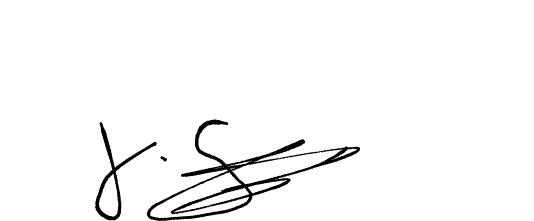
\includegraphics[height=2cm]{graphics/signature Final.png}\\
\end{tabular}
}
\end{tabular}
\begin{appendix} % Anhang
\section{Hardware-Informationen}
\label{hw-info}
Links zur verwendeten Hardware:
\begin{itemize}
    \item \href{https://de.aliexpress.com/item/32809373195.html?...}{Stift 1}
    \item \href{https://de.aliexpress.com/item/32809984821.html?...}{Stift 2}
    \item \href{https://de.aliexpress.com/item/4000575587804.html?...}{Filterfolie Typ 11}
    \item \href{https://realsenseai.com/stereo-depth-cameras/real-sense-depth-camera-d455/?wapkw=d455}{Intel Realsense D455}
\end{itemize}

\begin{figure}[H]
    \centering
    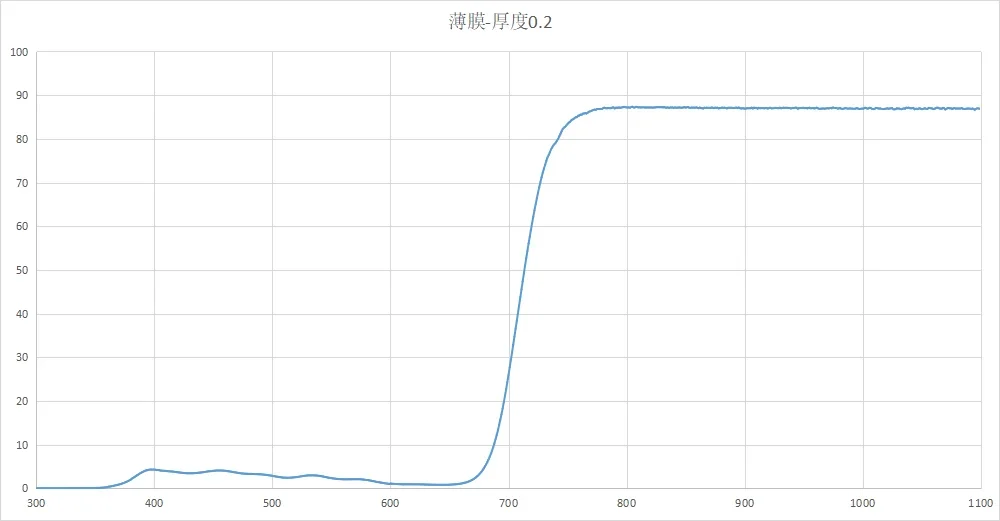
\includegraphics[width=0.5\linewidth]{graphics/filter_kurve.png}
    \caption{Filterkurve der Typ-11-Folie (X-Achse: Wellenlänge, Y-Achse: Dämpfung in \%)}
    \label{fig:filter_kurve}
\end{figure}
\section{Anleitung}
Dieser Abschnitt beschreibt die Funktion sämtlicher Buttons.

\begin{figure}[H]
    \centering
    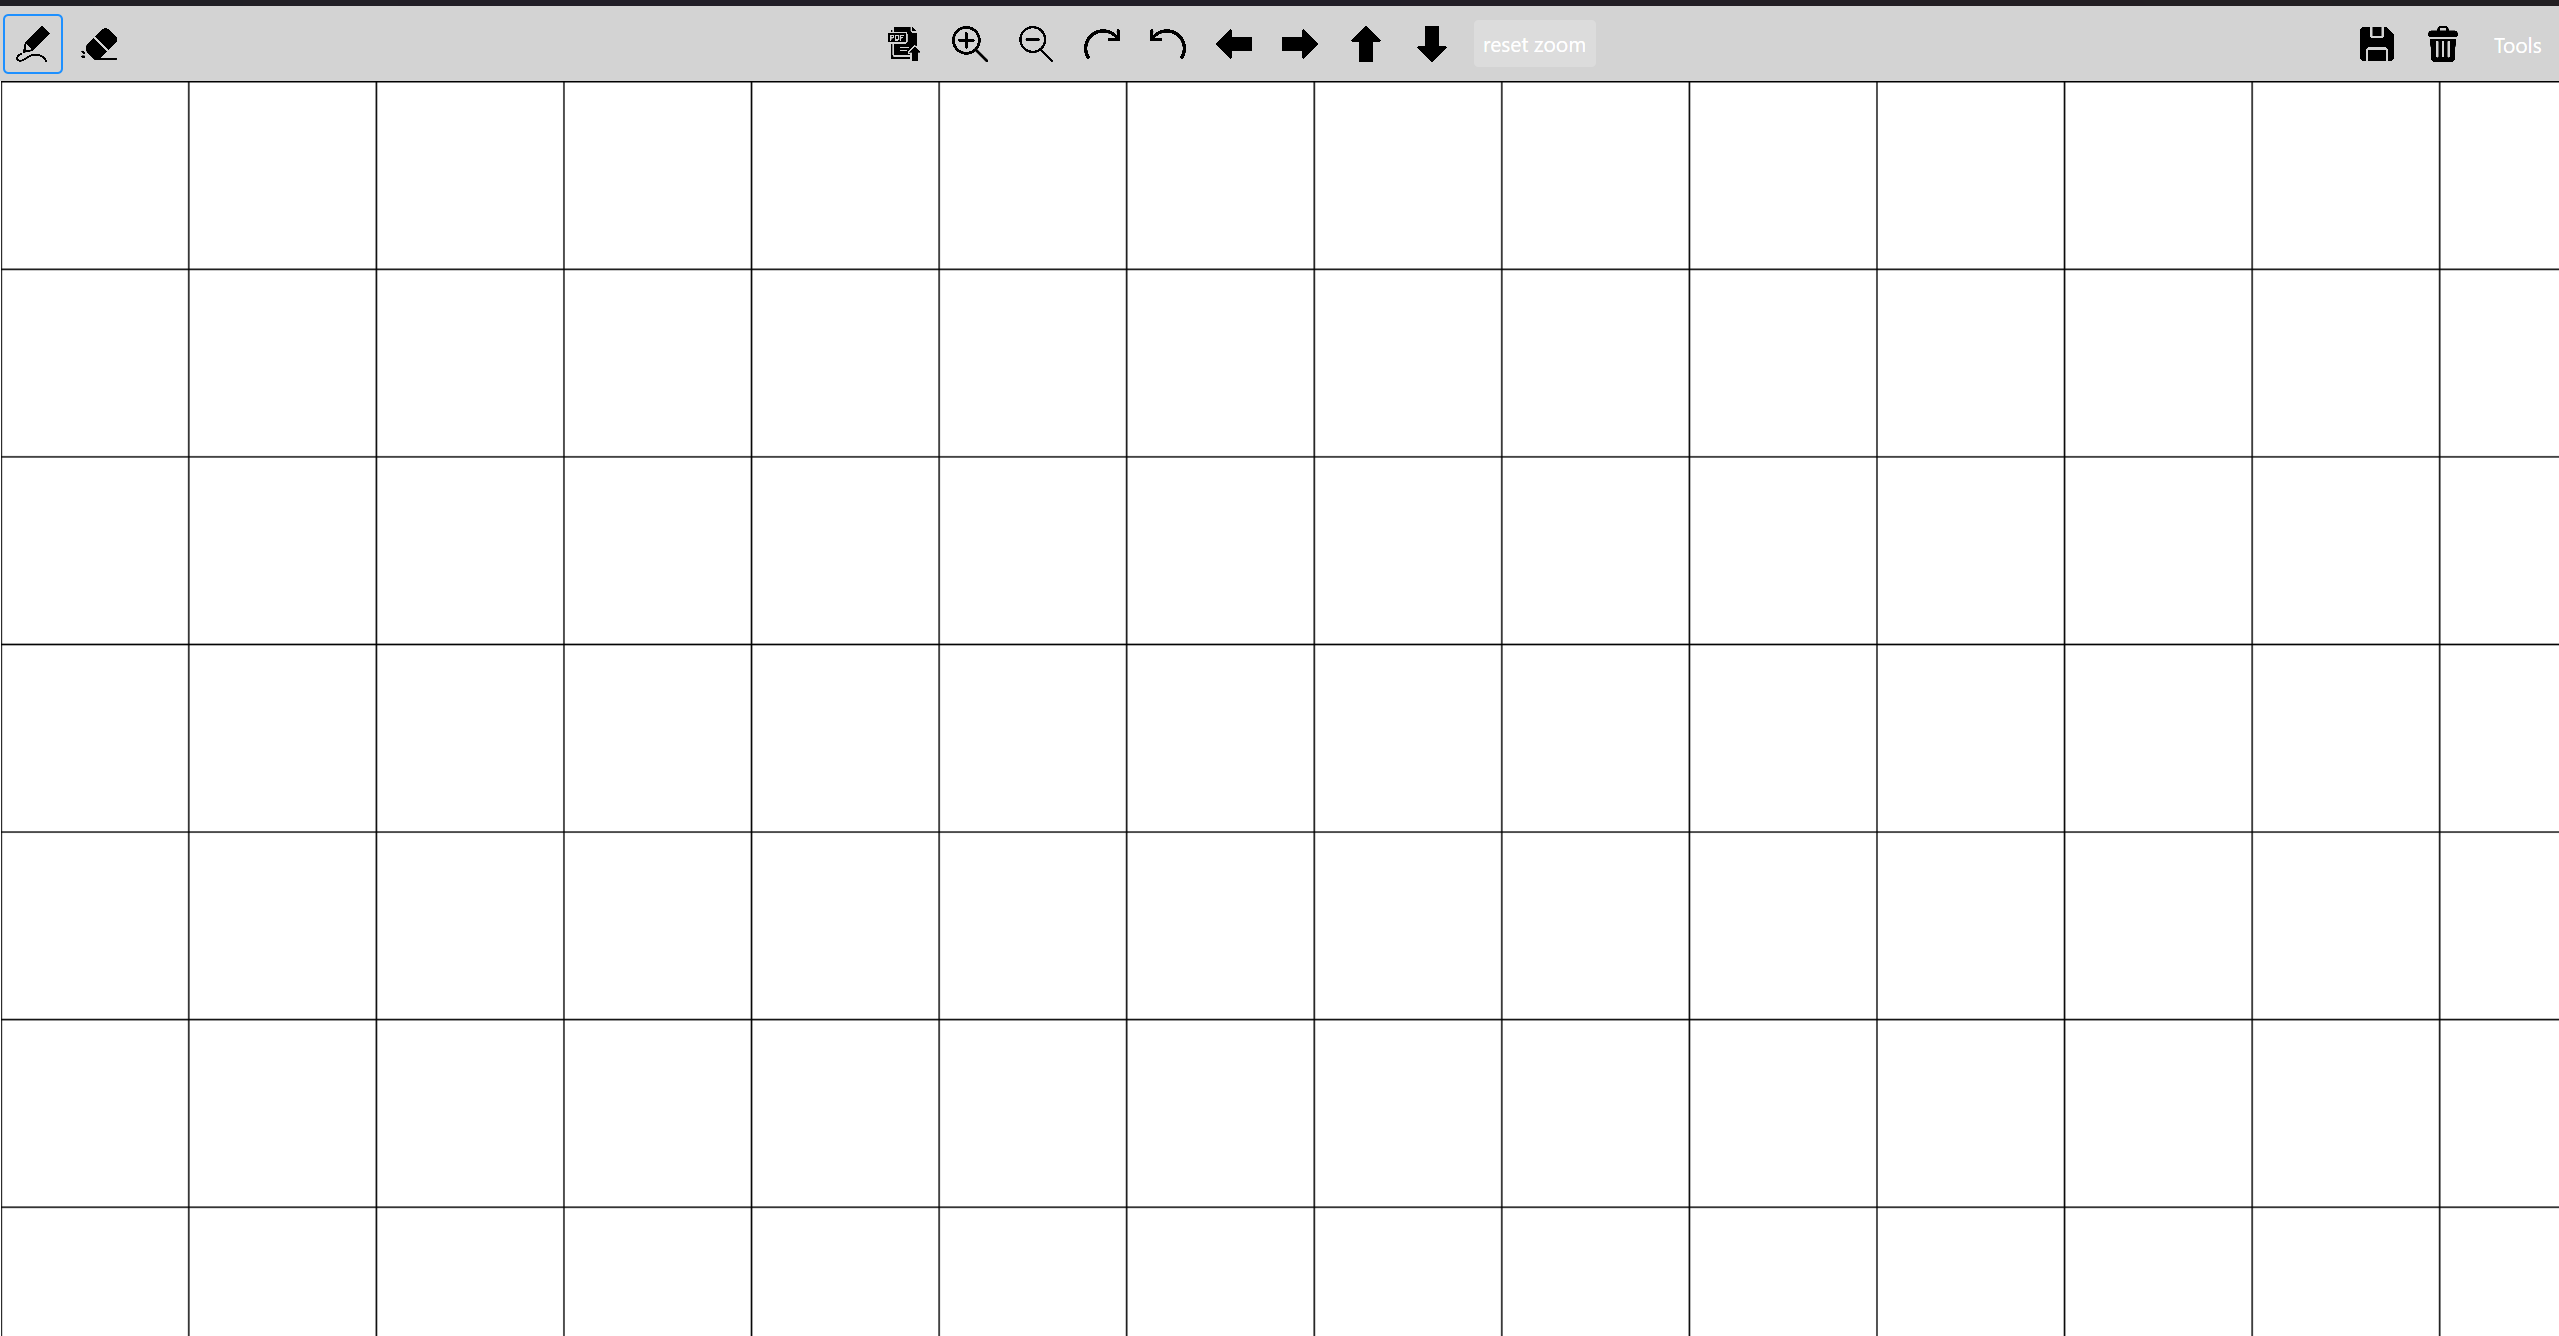
\includegraphics[width=0.5\linewidth]{graphics/ui_screenshot.png}
    \caption{Hauptansicht}
    \label{fig:ui_screenshot}
\end{figure}

Grundsätzlich sind die Funktionen wie folgt angeordnet:  
Links oben befinden sich die Werkzeuge, welche die Zeichenfunktionalität betreffen. In der Mitte sind alle Funktionen zur Steuerung der PDF-Lade- und -Anzeigeoptionen platziert. Rechts oben befinden sich die Buttons zum Löschen, Speichern sowie das Menü für Setup-Funktionen.

\subsection{Stiftfunktionen}
\begin{figure}[H]
    \centering
    
\includegraphics[width=0.5\linewidth]{graphics/stift_funktionen.png}
    \caption{Stiftfunktionen}
    \label{fig:stift_funktionen}
\end{figure}

Die Stiftfunktionen umfassen das Zeichnen sowie das Löschen an der Position des Stiftes. Der aktuell aktive Modus wird durch einen blauen Rahmen angezeigt.  
Das linke Symbol steht für den Schreibmodus mit dem Stift, während das rechte Symbol den Löschmodus aktiviert.  
Beim Anklicken des aktiven Symbols können verschiedene Optionen angepasst werden: die Strichdicke, die Radiergummigrösse sowie im Zeichenmodus zusätzlich die Stiftfarbe.

\begin{figure}[H]
    \begin{minipage}{0.48\textwidth}
        \centering
        \frame{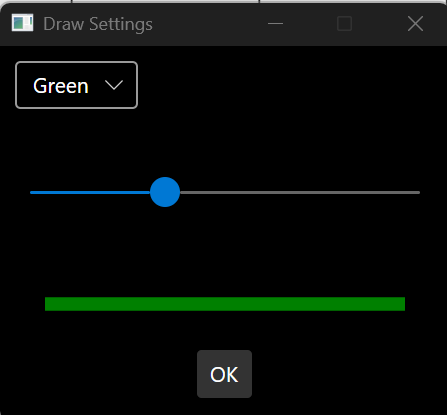
\includegraphics[width=0.9\linewidth]{graphics/draw_settings.png}}
        \caption{Zeichenmodus-Einstellungen}
        \label{fig:draw_settings}
    \end{minipage}
    \hfill
    \begin{minipage}{0.48\textwidth}
        \centering
        \frame{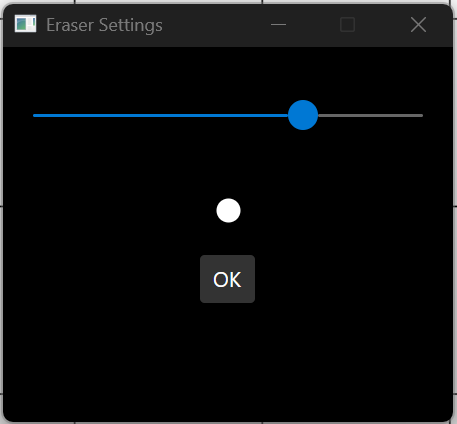
\includegraphics[width=0.9\linewidth]{graphics/eraser_settings.png}}
        \caption{Radiermodus-Einstellungen}
        \label{fig:eraser_settings}
    \end{minipage}
\end{figure}

\clearpage

\subsection{PDF-Lade- und Anzeigeoptionen}
\begin{figure}[H]
    \centering
    
\includegraphics[width=0.5\linewidth]{graphics/pdf_options.png}
    \caption{Bedienelemente für PDF-Lade- und Anzeigeoptionen}
    \label{fig:pdf_options}
\end{figure}

Die Buttons der PDF-Optionen haben – von links nach rechts – folgende Funktionen:
\begin{itemize}
    \item Öffnet den systemeigenen Dateiauswahldialog (Filepicker) und erlaubt die Auswahl eines PDF-Dokuments, das in der Zeichenfläche angezeigt werden soll.
    \item \emph{Zoom In}: Vergrössert den Inhalt der Zeichenfläche an der aktuellen Position.
    \item \emph{Zoom Out}: Verkleinert den Inhalt der Zeichenfläche an der aktuellen Position.
    \item Dreht den Inhalt der Zeichenfläche um 90° im Uhrzeigersinn.
    \item Dreht den Inhalt der Zeichenfläche um 90° gegen den Uhrzeigersinn.
    \item Bei aktivem Zoom: Verschiebt den Inhalt der Zeichenfläche nach links.
    \item Bei aktivem Zoom: Verschiebt den Inhalt der Zeichenfläche nach rechts.
    \item Bei aktivem Zoom: Verschiebt den Inhalt der Zeichenfläche nach oben.
    \item Bei aktivem Zoom: Verschiebt den Inhalt der Zeichenfläche nach unten.
    \item Setzt den Zoomfaktor sofort auf den Standardwert (0) zurück.
\end{itemize}
\section{Löschen, Speichern und Setup-Funktionen}
\begin{figure}[H]
    \centering
    
\includegraphics[width=0.5\linewidth]{graphics/setup_funktionen.png}
    \caption{Bedienelemente für Speichern, Löschen und Setup}
    \label{fig:setup_funktionen}
\end{figure}

Der Button auf der linken Seite öffnet den Datei-Explorer des Betriebssystems und erlaubt das Abspeichern des Inhalts der Zeichenfläche auf dem System.  
Der zweite Button von links löscht den gesamten Inhalt der Zeichenfläche und setzt diese auf den Zustand mit den Standardgitterlinien zurück.  
Der \emph{Tools}-Button öffnet ein Menü mit allen Funktionen rund um das Setup.

\begin{figure}[H]
    \centering
    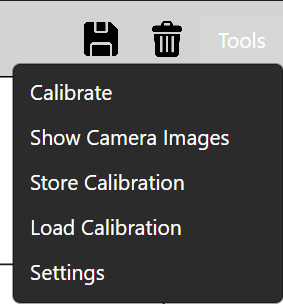
\includegraphics[width=0.5\linewidth]{graphics/toolsmenu.png}
    \caption{Tools-Menü}
    \label{fig:toolsmenu}
\end{figure}

Das Tools-Menü enthält folgende Funktionen:
\begin{itemize}
    \item \textbf{Calibrate}: Öffnet das Kalibrationsfenster, in dem nacheinander fünf rote Punkte mit dem Infrarotstift berührt werden müssen, um die Zeichenfläche zu kalibrieren.
    \begin{figure}[H]
        \centering
        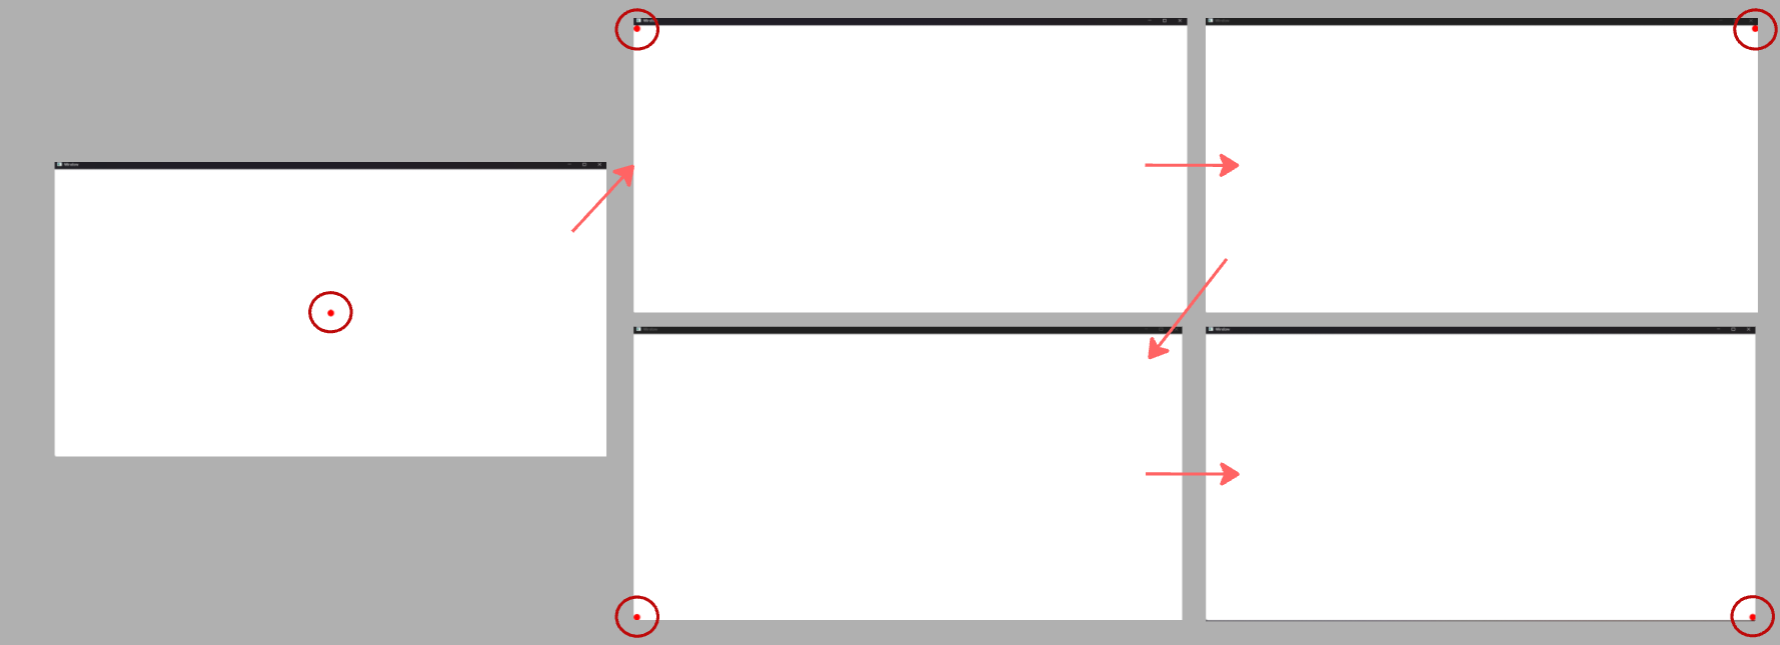
\includegraphics[width=0.5\linewidth]{graphics/ablauf_kalibration.png}
        \caption{Ablauf der Kalibration}
        \label{fig:ablauf_kalibration}
    \end{figure}
    \item \textbf{Show Camera Images}: Schaltet die Sichtbarkeit eines separaten Fensters um, in dem die Bilder der RGB- und Infrarotkamera sowie das Resultat der Binarisierung angezeigt werden.
    \item \textbf{Store Calibration}: Speichert die aktuelle Kalibration und die vorgenommenen Einstellungen.
    \item \textbf{Load Calibration}: Lädt die zuletzt gespeicherte Kalibration und Einstellungen.
    \item \textbf{Settings}: Öffnet das Einstellungsmenü.
\end{itemize}

\begin{figure}[H]
    \centering
    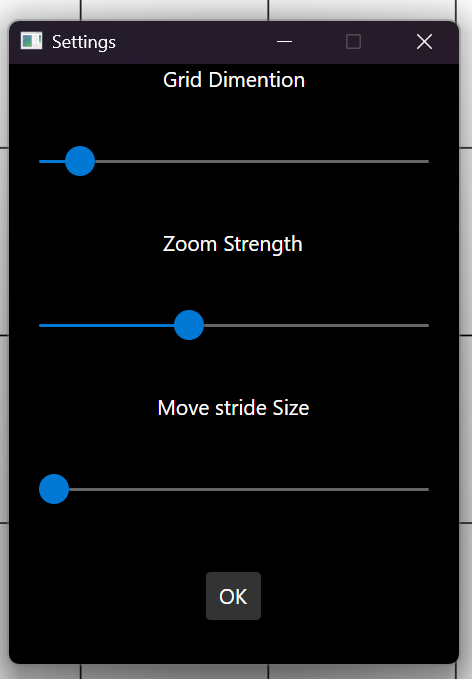
\includegraphics[width=0.5\linewidth]{graphics/settings_window.png}
    \caption{Einstellungsfenster}
    \label{fig:settings_window}
\end{figure}

Im Einstellungsmenü sind folgende Optionen verfügbar:
\begin{itemize}
    \item \textbf{Grid Dimension}: Legt die Grösse des Gitternetzes fest.
    \item \textbf{Zoom Strength}: Bestimmt, wie stark bei einem Klick hinein- oder herausgezoomt wird.
    \item \textbf{Move Stride Size}: Legt fest, um welchen Betrag der Inhalt der Zeichenfläche pro Klick verschoben wird.
\end{itemize}
\clearpage
\section{Interviewauswertung mit dem Kunden – Feldtest}

Im Anschluss an den Feldtest wurde ein qualitatives Interview mit einem Vertreter des SCDH durchgeführt. Ziel war es, die Perspektive der Auftraggeberseite hinsichtlich Integration, Nutzen und möglicher Weiterentwicklungen des Systems zu erfassen.

\subsection{Integration in bestehende Workshop-Formate}

\textbf{Frage:} Wie gut lässt sich das aktuelle System in Ihre bestehenden Workshop-Formate integrieren?

\textbf{Antwort:}
\begin{itemize}
    \item Das System bewegt sich technisch in die richtige Richtung.
    \item Die Integration mit bestehenden PDF-Workflows funktioniert bereits gut.
    \item Details zum Workshop-Ablauf müssen noch abgestimmt werden.
    \item Insgesamt zeigt sich ein vielversprechendes Potenzial mit klar reaktiver Nutzung im Vergleich zu bestehenden Methoden.
\end{itemize}

\subsection{Grösster Nutzen für den Arbeitsalltag}

\textbf{Frage:} Wo sehen Sie den grössten Nutzen dieses Systems für Ihre tägliche Arbeit?

\textbf{Antwort:}
\begin{itemize}
    \item Möglichkeit, Änderungen am Plan reaktiv vorzunehmen – grosser Gewinn.
    \item Arbeit mit einer leeren Zeichenfläche (vergleichbar mit weissem Papier) ermöglicht kreative Freiheit.
\end{itemize}

\subsection{Potenzial für andere Zielgruppen}

\textbf{Frage:} Welche Anwendungsfälle oder Zielgruppen könnten von einer Weiterentwicklung profitieren?

\textbf{Antwort:}
\begin{itemize}
    \item Architekt:innen, da viele Kommunikationsschleifen (E-Mails, Telefonate) wegfallen.
    \item Stadtverwaltung (z.B. Planung öffentlicher Räume, Parkplätze).
    \item Brainstorming-Tool oder technische Planungen (z.B. Elektriker:innen, Techniker:innen).
\end{itemize}

\subsection{Voraussetzungen für produktiven Einsatz}

\textbf{Frage:} Welche Voraussetzungen müsste das System erfüllen, um produktiv eingesetzt werden zu können?

\textbf{Antwort:}
\begin{itemize}
    \item Unterstützung mehrerer Displays und Spiegelfunktion.
    \item Zuverlässige und exakte Kalibrierung (1:1).
    \item Durchdachtes Setup (Installationsort, Abläufe).
    \item Aktuelle Funktionen sind bereits brauchbar für Workshops.
    \item Einsatz von zwei IR-Kameras könnte Vorteile bringen.
    \item Import von Plänen ist essenziell und funktioniert gut.
\end{itemize}

\subsection{Gewünschte Funktionen und Erweiterungen}

\textbf{Frage:} Welche Funktionen oder Erweiterungen wünschen Sie sich für eine zukünftige Version?

\textbf{Antwort:}
\begin{itemize}
    \item QR-Codes zur Visualisierung von Objekten (z.B. Bett, Stuhl).
    \item Objektkatalog zur schnellen Auswahl und Platzierung.
    \item Möglichkeit zur Remote-Zusammenarbeit.
    \item Reset-Buttons für 0\% und 100\%-Zoom.
    \item Undo-/Redo-Funktion.
    \item Kommentarfunktion via Post-its oder Textfelder.
\end{itemize}

\subsection{Herausforderungen bei der Einführung}

\textbf{Frage:} Welche Herausforderungen sehen Sie bei der Einführung eines solchen Systems in der Praxis?

\textbf{Antwort:}
\begin{itemize}
    \item Hardwarebeschaffung (Stift, Projektor etc.).
    \item Planung des Setups: Wo und wie wird aufgebaut?
    \item Integration in bestehende Softwareumgebungen könnte komplex werden.
\end{itemize}

\subsection{Weitere Rückmeldungen}

\textbf{Frage:} Gibt es sonstige Rückmeldungen oder Verbesserungsvorschläge, die Sie uns mitgeben möchten?

\textbf{Antwort:}
\begin{itemize}
    \item Keine weiteren Vorschläge.
    \item Positives Feedback: Die Mitwirkung des Projektteams wurde sehr geschätzt.
\end{itemize}
\clearpage
\section{Testaufbau und Szenario}
Die Usability-Tests wurden anhand des Szenarios \emph{Hospital Planning} durchgeführt. 
Die Testpersonen sollten in einem simulierten Planungsmeeting die Position eines Tisches in \textbf{BEDROOM3} vorschlagen, Änderungen nach Feedback der Architekt:in umsetzen und abschliessend den Plan speichern.

\textbf{Aufgabenabfolge:}
\begin{enumerate}
    \item Zwei Minuten freies Zeichnen
    \item Zeichnung komplett löschen
    \item PDF mit Grundriss (\texttt{Hospital\_Floor\_Plan.pdf}) hochladen
    \item Stiftfarbe auf Rot ändern
    \item Tisch links vom Bett in BEDROOM3 einzeichnen
    \item Nach Feedback: Tisch löschen und rechts vom Bett platzieren
    \item Tischmasse 1\,m $\times$ 1\,m skizzieren und Beschriftung \enquote{table} in den Tisch einfügen(nicht massstabsgetreu erforderlich)
    \item Plan lokal speichern
\end{enumerate}

\begin{center}
    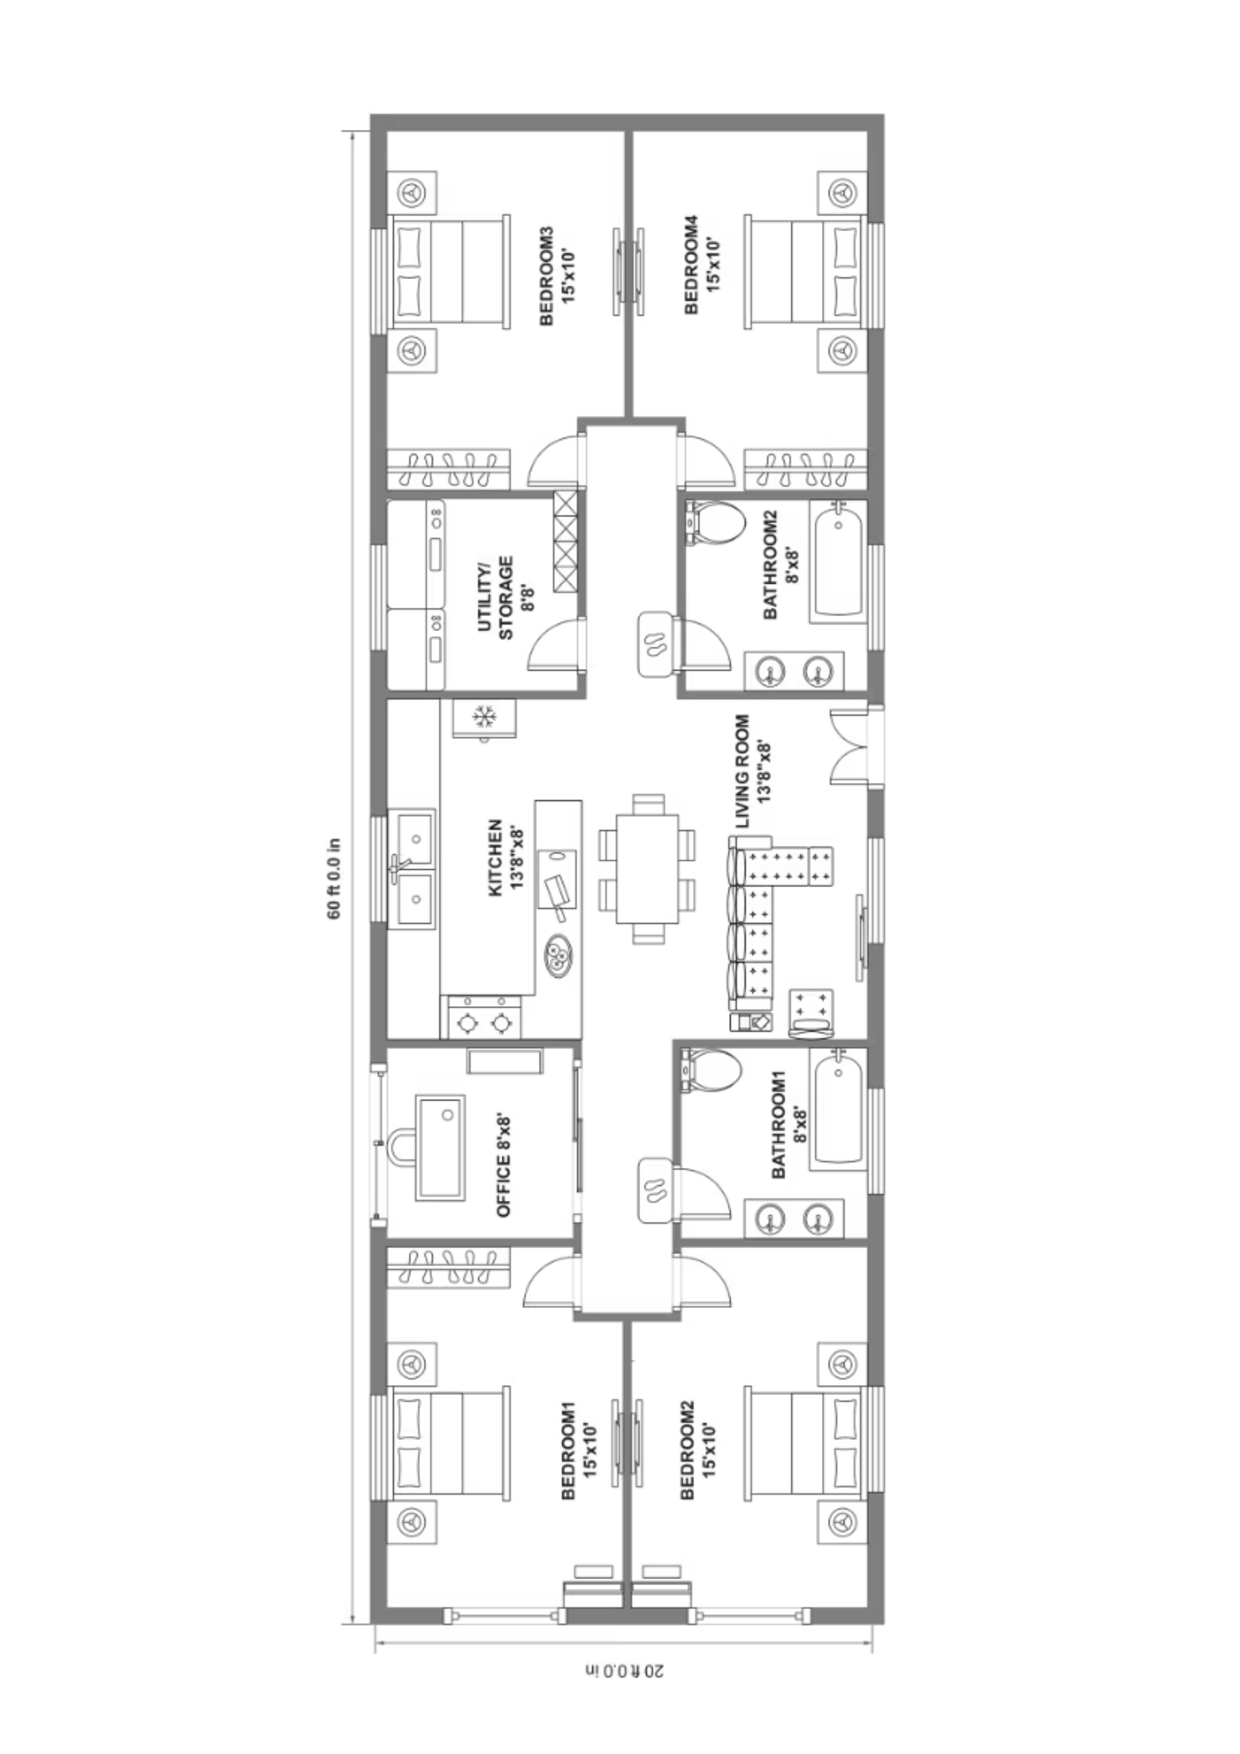
\includegraphics[width=0.65\textwidth]{graphics/Hospital_Floor_Plan.pdf}
    \captionof{figure}{Verwendeter Grundrissplan \texttt{Hospital\_Floor\_Plan.pdf}}
\end{center}
\clearpage

\textbf{SUS-Fragebogen:}  
Nach Abschluss der Aufgaben wurde jeder Testperson der standardisierte \emph{System Usability Scale} (SUS) Fragebogen vorgelegt.

\begin{center}
    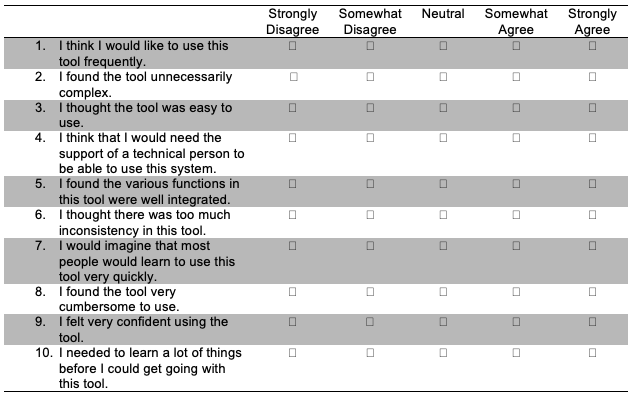
\includegraphics[width=0.95\textwidth]{graphics/sus_blank.png}
    \captionof{figure}{Leerer SUS-Fragebogen (10 Aussagen, 5-stufige Skala von \enquote{Strongly Disagree} bis \enquote{Strongly Agree})}
\end{center}

\textbf{Follow-up-Fragen:}  
Nach der SUS-Bewertung wurden zusätzlich folgende offenen Fragen gestellt:
\begin{enumerate}
    \item \textbf{Was hat Ihnen am Tool am besten gefallen?}
    \item \textbf{Gab es etwas, das verwirrend oder schwierig zu bedienen war?}
    \item \textbf{Fehlt etwas, das Sie erwartet oder gerne gehabt hätten?}
    \item \textbf{Haben Sie Vorschläge, wie das Tool verbessert werden könnte?}
\end{enumerate}

\clearpage

\section{Testergebnisse}
\subsection{Person 1 – SUS 67{,}5}
\textbf{Zur Person:}\\
ICompetence-Student, 27 Jahre alt\\

\textbf{Beobachtung:}
\begin{enumerate}
    \item Zeichnen Sie frei für etwa 2 Minuten.
    \begin{itemize}
        \item Nutzer wollte den «Rotate»-Button verwenden, um eine Aktion rückgängig zu machen.
        \item Handhabung des Stifts wurde als gewöhnungsbedürftig empfunden.
        \item Erkenntnis, dass die Kamera nicht zuverlässig erfasst, wenn die Hand den Stift verdeckt.
        \item Bessere Erkennung, wenn der Stift weiter hinten gehalten wird – jedoch ungewohnt.
        \item Positives Feedback: «Fühlt sich wie ein Stift an, wenn es funktioniert.»
        \item Unsicherheit, wie vorzugehen ist, wenn Striche nicht korrekt erkannt werden.
        \item Wunsch nach einem dünneren, spitzeren Stift für präziseres Zeichnen.
    \end{itemize}

    \item Löschen Sie Ihre Zeichnung vollständig.
    \begin{itemize}
        \item «Rotation»-Button wurde mit «Rückgängig»-Button verwechselt.
    \end{itemize}

    \item Laden Sie die PDF-Datei mit dem Grundriss \texttt{Hospital\_Floor\_Plan.pdf} hoch.
    \begin{itemize}
        \item Versuch, Text einzugeben anstatt eine Datei auszuwählen.
        \item PDF-Icon mit Pfeil nach aussen wurde als «Exportieren»-Symbol interpretiert.
    \end{itemize}

    \item Ändern Sie die Stiftfarbe auf Rot.
    \begin{itemize}
        \item Unklar, wo die Funktion zu finden ist.
        \item Slider zur Farbauswahl wurde bewegt, jedoch mit Problemen.
    \end{itemize}

    \item Suchen Sie \texttt{BEDROOM3} und zeichnen Sie einen Tisch links vom Bett.
    \begin{itemize}
        \item Architekt gab an, dass diese Position nicht möglich ist.
    \end{itemize}

    \item Radieren Sie den Tisch und zeichnen Sie ihn rechts vom Bett.
    \begin{itemize}
        \item Unsicherheit, ob der Radiergummi-Modus aktiviert war.
    \end{itemize}

    \item Zeichnen Sie die Abmessungen 1\,m $\times$ 1\,m und schreiben Sie «table» hinein.
    \begin{itemize}
        \item Zoom wird als nicht optimal beschrieben, vermutlich nicht genutzt.
        \item Verschiebung (Pan) nur in kleinen und langsamen Schritten möglich.
        \item Versuch, durch Gedrückthalten zu verschieben.
    \end{itemize}

    \item Speichern Sie den Plan auf Ihrem Laptop.
    \begin{itemize}
        \item Kein Dateiname angegeben, daher Standardname verwendet.
        \item Speichervorgang ohne Rückmeldung – Bestätigung (z. B. Balken mit «Saved» oder Ordner-Öffnen-Option) wäre wünschenswert.
    \end{itemize}
\end{enumerate}

\clearpage

\textbf{SUS-Antworten:}
\begin{center}
    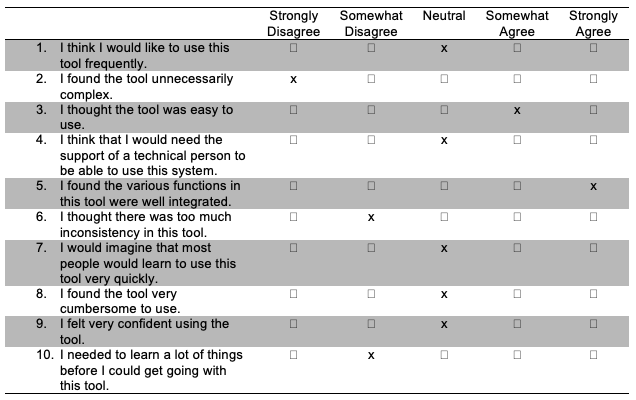
\includegraphics[width=0.95\textwidth]{graphics/sus_person1.png}
\end{center}

\textbf{Follow-up:}
\begin{enumerate}
    \item \textbf{Was hat Ihnen am Tool am besten gefallen?}
    \begin{itemize}
        \item Möglichkeit, PDF-Dateien hochzuladen und zu bearbeiten.
        \item Farb- und Stiftdickenänderung möglich.
        \item Speichern der Arbeit.
    \end{itemize}

    \item \textbf{Gab es etwas, das verwirrend oder schwierig zu bedienen war?}
    \begin{itemize}
        \item Verständnis der Zeichenfunktion.
    \end{itemize}

    \item \textbf{Fehlt etwas, das Sie erwartet oder gerne gehabt hätten?}
    \begin{itemize}
        \item Undo-Button.
        \item Speichern mit klarer Bestätigung, dass die Datei gesichert wurde.
        \item PDF-Icon nicht eindeutig.
    \end{itemize}

    \item \textbf{Haben Sie Vorschläge, wie das Tool verbessert werden könnte?}
    \begin{itemize}
        \item Anpassung der Kameraposition für besseres Zeichnen.
        \item Blaue Farbe wirkt wie Schwarz.
        \item Beim Verschieben des Plans wird auch die Zeichnung verschoben.
        \item Zusätzlicher Button für schnellen Farbwechsel.
    \end{itemize}
\end{enumerate}
\clearpage
\subsection{Person 2 – SUS SUS 85{,}0}
\textbf{Zur Person:}\\
Architektin, 62 Jahre alt\\

\textbf{Beobachtung:}
\begin{enumerate}
    \item Zeichnen Sie frei für etwa 2 Minuten.
    \begin{itemize}
        \item Nach dem Ansetzen des Stifts dauerte es einen kurzen Moment, bis das System reagierte, wodurch der Punkt nicht exakt dort erschien, wo sich die Stiftspitze befand.
        \item Geschwindigkeit beeinträchtigte die Genauigkeit.
        \item Insgesamt gutes Feedback, insbesondere wenn dem System etwas Zeit gegeben wird.
    \end{itemize}

    \item Löschen Sie Ihre Zeichnung vollständig.
    \begin{itemize}
        \item Keine Probleme.
    \end{itemize}

    \item Laden Sie die PDF-Datei mit dem Grundriss \texttt{Hospital\_Floor\_Plan.pdf} hoch.
    \begin{itemize}
        \item Kein Problem beim Hochladen.
        \item Kommentar: Bedienung erfordert CAD-Erfahrung. Der verwendete Button war das einzige Symbol, das selbsterklärend wirkte.
        \item Nicht selbstverständlich für unerfahrene Nutzer:innen.
        \item Nachfrage der Testperson: «Kann ich jetzt Wände verschieben?»
    \end{itemize}

    \item Ändern Sie die Stiftfarbe auf Rot.
    \begin{itemize}
        \item Kommentar: «Gut kann ich Englisch.»
    \end{itemize}

    \item Suchen Sie \texttt{BEDROOM3} und zeichnen Sie einen Tisch links vom Bett.
    \begin{itemize}
        \item Keine Probleme.
    \end{itemize}

    \item Radieren Sie den Tisch und zeichnen Sie ihn rechts vom Bett.
    \begin{itemize}
        \item Reaktion: Am falschen Ort schreiben funktioniert nicht.
    \end{itemize}

    \item Zeichnen Sie die Abmessungen 1\,m $\times$ 1\,m und schreiben Sie «table» hinein.
    \begin{itemize}
        \item Keine Probleme.
    \end{itemize}

    \item Speichern Sie den Plan auf Ihrem Laptop.
    \begin{itemize}
        \item Keine Probleme.
    \end{itemize}
\end{enumerate}

\clearpage

\textbf{SUS-Antworten (Bild):}
\begin{center}
    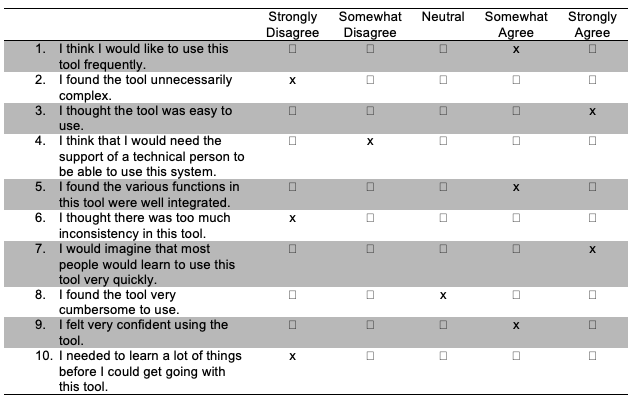
\includegraphics[width=0.95\textwidth]{graphics/sus_person2.png}
\end{center}

\textbf{Follow-up:}
\begin{enumerate}
    \item \textbf{Was hat Ihnen am Tool am besten gefallen?}
    \begin{itemize}
        \item Einfaches Umschalten zwischen Funktionen.
        \item Radiergummi funktioniert gut; Wunsch: einzelne Striche gezielt löschen können.
    \end{itemize}

    \item \textbf{Gab es etwas, das verwirrend oder schwierig zu bedienen war?}
    \begin{itemize}
        \item Nein.
        \item Kommentar: Funktion zum einfachen Wechseln zwischen Plänen und Dokumenten wurde nicht ausprobiert; als Architekt wäre dies wünschenswert.
    \end{itemize}

    \item \textbf{Fehlt etwas, das Sie erwartet oder gerne gehabt hätten?}
    \begin{itemize}
        \item Nein.
    \end{itemize}

    \item \textbf{Haben Sie Vorschläge, wie das Tool verbessert werden könnte?}
    \begin{itemize}
        \item Verschiedene Pläne überlagern.
        \item Wechsel zwischen Plänen ohne vorheriges Speichern ermöglichen.
    \end{itemize}
\end{enumerate}

\clearpage

\subsection{Person 3 – SUS 85,0}
\textbf{Zur Person:}\\
Medizin-Student, 24 Jahre alt

\textbf{Beobachtung:}
\begin{enumerate}
\item Zeichnen Sie frei für etwa 2 Minuten.
\begin{itemize}
\item Präzision meist sehr gut; kleinere Probleme beim Setup mit Doppel-Erkennung.
\item Leichter Delay, aber nicht gravierend.
\item Schrift problemlos.
\end{itemize}

\item Löschen Sie Ihre Zeichnung vollständig.
\begin{itemize}
    \item Alles löschen problemlos; selbsterklärend.
\end{itemize}

\item Laden Sie die PDF-Datei mit dem Grundriss \texttt{Hospital\_Floor\_Plan.pdf} hoch.
\begin{itemize}
    \item Alles problemlos.
\end{itemize}

\item Ändern Sie die Stiftfarbe auf Rot.
\begin{itemize}
    \item Funktion bereits beim freien Zeichnen allerdings nicht absichtlich; Änderung eventuell Drop-down-Indikator wünschenswert.
\end{itemize}

\item Suchen Sie \texttt{BEDROOM3} und zeichnen Sie einen Tisch links vom Bett.
\begin{itemize}
    \item Funktion ausgeführt; kleinere Probleme wegen Bugs in den PDF-Controls.
\end{itemize}

\item Radieren Sie den Tisch und zeichnen Sie ihn rechts vom Bett.
\begin{itemize}
    \item Gewohnt von iPad: PDF-Linie, Radiergummi und Smart-Eraser Funktion.
    \item Sonst alles ok.
\end{itemize}

\item Zeichnen Sie die Abmessungen 1\,m $\times$ 1\,m und schreiben Sie «table» hinein.
\begin{itemize}
    \item Keine Probleme.
\end{itemize}

\item Speichern Sie den Plan auf Ihrem Laptop.
\begin{itemize}
    \item Keine Probleme.
\end{itemize}
\end{enumerate}

\clearpage

\textbf{SUS-Antworten (Bild):}
\begin{center}
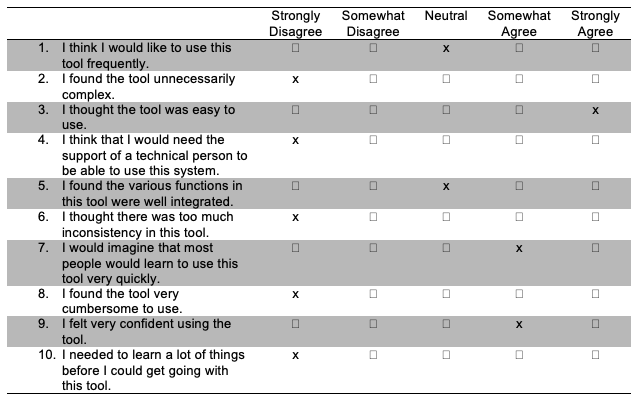
\includegraphics[width=0.95\textwidth]{graphics/sus_person3.png}
\end{center}

\textbf{Follow-up:}  
\begin{enumerate}
    \item \textbf{Was hat Ihnen am Tool am besten gefallen?}
    \begin{itemize}
        \item Freiheit, auf beliebiger Fläche zu zeichnen und damit verbundene Flexibilität.
    \end{itemize}

    \item \textbf{Gab es etwas, das verwirrend oder schwierig zu bedienen war?}
    \begin{itemize}
        \item Tracking-Fehler (Zacken-Bug).
        \item PDF-Controls teilweise verwirrend.
        \item Reset-Button löscht PDF-Elemente mit.
    \end{itemize}

    \item \textbf{Fehlt etwas, das Sie erwartet oder gerne gehabt hätten?}
    \begin{itemize}
        \item Rückgängig-Funktion (Undo).
        \item Wiederherstellen-Funktion.
        \item Lasso-Löschen, Duplizieren und Verschieben von Elementen.
        \item Touch-Input-Unterstützung.
    \end{itemize}

    \item \textbf{Haben Sie Vorschläge, wie das Tool verbessert werden könnte?}
    \begin{itemize}
        \item Bessere Projektion der Unterlagen.
        \item Details besser lesbar machen (bedingt durch Setup).
        \item Fehlende Funktionen, die erwartet werden, implementieren (z.B. Undo, Lasso, Duplizieren).
    \end{itemize}
\end{enumerate}

\clearpage
\subsection{Person 4 – SUS 70}  
\textbf{Zur Person:}\\
Medizin-Studentin, 24 Jahre alt 

\textbf{Beobachtung:}  
\begin{enumerate}
    \item Zeichnen Sie frei für etwa 2 Minuten.
    \begin{itemize}
        \item Pen-Einstellungen nicht klar.
        \item PDF-Control-Icons nicht intuitiv.
        \item Undo-Button fehlt.
    \end{itemize}

    \item Löschen Sie Ihre Zeichnung vollständig.
    \begin{itemize}
        \item Kein intuitiver Button vorhanden.
    \end{itemize}

    \item Laden Sie die PDF-Datei mit dem Grundriss hoch.
    \begin{itemize}
        \item Keine Probleme.
    \end{itemize}

    \item Ändern Sie die Stiftfarbe auf Rot.
    \begin{itemize}
        \item Klar nach Aufgabenstellung, keine Probleme.
    \end{itemize}

    \item Suchen Sie \texttt{BEDROOM3} und zeichnen Sie einen Tisch links vom Bett.
    \begin{itemize}
        \item Keine Probleme.
    \end{itemize}

    \item Radieren Sie den Tisch und zeichnen Sie ihn rechts vom Bett.
    \begin{itemize}
        \item Am Anfang Zickzack-Bug, danach keine Probleme.
    \end{itemize}

    \item Zeichnen Sie die Abmessungen 1\,m $\times$ 1\,m und schreiben Sie «table» hinein.
    \begin{itemize}
        \item Keine Probleme.
    \end{itemize}

    \item Speichern Sie den Plan auf Ihrem Laptop.
    \begin{itemize}
        \item Keine Probleme.
    \end{itemize}
\end{enumerate}

\clearpage

\textbf{SUS-Antworten (Bild):}
\begin{center}
    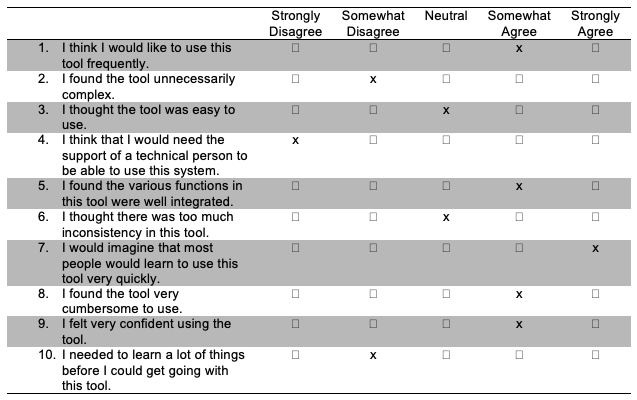
\includegraphics[width=0.95\textwidth]{graphics/sus_person4.png}
\end{center}

\textbf{Follow-up:}  
\begin{enumerate}
    \item \textbf{Was hat Ihnen am Tool am besten gefallen?}
    \begin{itemize}
        \item Dateihandling einfach zu bedienen, ohne viel Klicken.
    \end{itemize}

    \item \textbf{Gab es etwas, das verwirrend oder schwierig zu bedienen war?}
    \begin{itemize}
        \item Zickzack-Bug beim Zeichnen.
        \item Undo-Button fehlt.
    \end{itemize}

    \item \textbf{Fehlt etwas, das Sie erwartet oder gerne gehabt hätten?}
    \begin{itemize}
        \item Undo-Button.
        \item Finger-Touch-Support.
        \item Drei Modi, um das Dokument zu verschieben; aktuelle Buttons umständlich.
    \end{itemize}

    \item \textbf{Haben Sie Vorschläge, wie das Tool verbessert werden könnte?}
    \begin{itemize}
        \item „Premium Feature“: automatische Formgenerierung (z.B. Quadrat 1\,m x 1\,m in Fläche ziehen).
        \item Verschieben von Zeichnungen.
        \item Hintergrund sollte nicht mit Radiert werden – aktuell unintuitiv.
    \end{itemize}
\end{enumerate}

\clearpage

\subsection{Person 5 – SUS 87.5}  
\textbf{Zur Person:}\\
IT-Projektmanager, 59 Jahre alt  

\textbf{Beobachtung:}  
\begin{enumerate}
    \item Zeichnen Sie frei für etwa 2 Minuten.
    \begin{itemize}
        \item Suchte vordefinierte Formen.
        \item Frage: Wiso gümmelt es den Hintergrund?.
        \item Bug: Stift-Menü geöffnet → keine direkte Anpassung möglich; Stift erscheint immer zuerst blau.
    \end{itemize}

    \item Löschen Sie Ihre Zeichnung vollständig.
    \begin{itemize}
        \item Kein Problem.
    \end{itemize}

    \item Laden Sie die PDF-Datei mit dem Grundriss hoch.
    \begin{itemize}
        \item Nur ein Button vorhanden, unklar, ob für Öffnen oder Exportieren.
    \end{itemize}

    \item Ändern Sie die Stiftfarbe auf Rot.
    \begin{itemize}
        \item Kein Problem, bereits vorher herausgefunden.
        \item Leichte Offsets beim Zeichnen.
    \end{itemize}

    \item Suchen Sie \texttt{BEDROOM3} und zeichnen Sie einen Tisch links vom Bett.
    \begin{itemize}
        \item Kein Problem.
    \end{itemize}

    \item Radieren Sie den Tisch und zeichnen Sie ihn rechts vom Bett.
    \begin{itemize}
        \item Verschiebe-Offset-Problem; Zoom nötig.
        \item Selektion- und Verschiebe-Tool wäre hilfreich.
        \item Wunsch nach Form-Katalog (Tische, Stühle etc.).
    \end{itemize}

    \item Zeichnen Sie die Abmessungen 1\,m $\times$ 1\,m und schreiben Sie «table» hinein.
    \begin{itemize}
        \item Schreiben auf Tisch: Schriftgrösse nicht optimal, zu klein + Offset beim genauen Einzeichnen.
    \end{itemize}

    \item Speichern Sie den Plan auf Ihrem Laptop.
    \begin{itemize}
        \item Kein Problem.
    \end{itemize}
\end{enumerate}

\clearpage

\textbf{SUS-Antworten (Bild):}
\begin{center}
    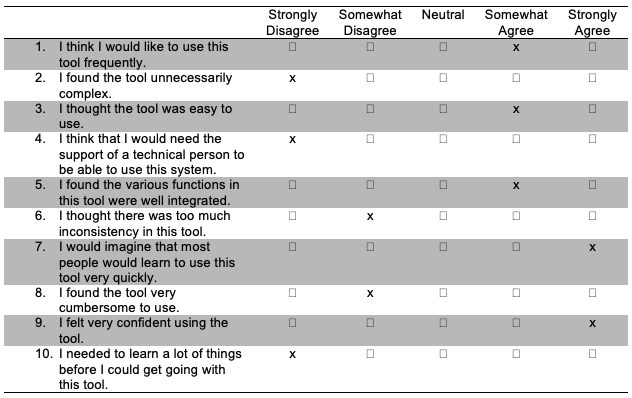
\includegraphics[width=0.95\textwidth]{graphics/sus_person5.png}
\end{center}

\textbf{Follow-up:}  
\begin{enumerate}
    \item \textbf{Was hat Ihnen am Tool am besten gefallen?}
    \begin{itemize}
        \item Grosse Stifte auf dem Tisch nutzen, Möglichkeit für Team-Planungsdiskussionen.
    \end{itemize}

    \item \textbf{Gab es etwas, das verwirrend oder schwierig zu bedienen war?}
    \begin{itemize}
        \item Offsets beim Zeichnen (vor allem beim Zoomen).  
        \item Hintergrund „gümmelet“ → suboptimal zum Arbeiten.
    \end{itemize}

    \item \textbf{Fehlt etwas, das Sie erwartet oder gerne gehabt hätten? / Verbesserungsvorschläge}
    \begin{itemize}
        \item Form-Katalog (Stühle, Tische, etc.)  
        \item Bereiche/Objekte verschieben und kopieren  
        \item Druckfunktion vom oberen Button integrieren  
        \item Mit einem grösseren Tisch sollte das Präzisionsproblem weniger auffallen
    \end{itemize}
\end{enumerate}

\clearpage

\subsection{Person 6 – SUS 85}  
\textbf{Zur Person:}\\
Logistikmitarbeiterin, 65 Jahre alt  

\textbf{Beobachtung:}  
\begin{enumerate}
    \item Zeichnen Sie frei für etwa 2 Minuten.
    \begin{itemize}
        \item Kein Problem.
    \end{itemize}

    \item Löschen Sie Ihre Zeichnung vollständig.
    \begin{itemize}
        \item Rotieren als Undo verwechselt.  
        \item Trash-Icon nicht gesehen.
    \end{itemize}

    \item Laden Sie die PDF-Datei mit dem Grundriss hoch.
    \begin{itemize}
        \item Zuerst in Windows-Taskleiste geschaut.  
        \item Danach klar und kein Problem.
    \end{itemize}

    \item Ändern Sie die Stiftfarbe auf Rot.
    \begin{itemize}
        \item Hat Radiergummi ausgewählt, da gedacht, Stift würde Schrift öffnen.
    \end{itemize}

    \item Suchen Sie \texttt{BEDROOM3} und zeichnen Sie einen Tisch links vom Bett.
    \begin{itemize}
        \item Sucht nach einem Symbol, um Tisch einzufügen.  
        \item Nach kleiner Anweisung kein Problem.
    \end{itemize}

    \item Radieren Sie den Tisch und zeichnen Sie ihn rechts vom Bett.
    \begin{itemize}
        \item Findet es nicht schön, dass Hintergrund „mitgegümmelt“ wird.  
        \item Sehr kleiner Tisch gezeichnet, Problem beim genauen Beschriften.  
    \end{itemize}

    \item Zeichnen Sie die Abmessungen 1\,m $\times$ 1\,m und schreiben Sie «table» hinein.
    \begin{itemize}
        \item Schreiben bei Aufgabe 1 ging bereits gut.
        \item Kein Problem.
    \end{itemize}

    \item Speichern Sie den Plan auf Ihrem Laptop.
    \begin{itemize}
        \item Kein Problem.
    \end{itemize}
\end{enumerate}

\clearpage

\textbf{SUS-Antworten (Bild):}
\begin{center}
    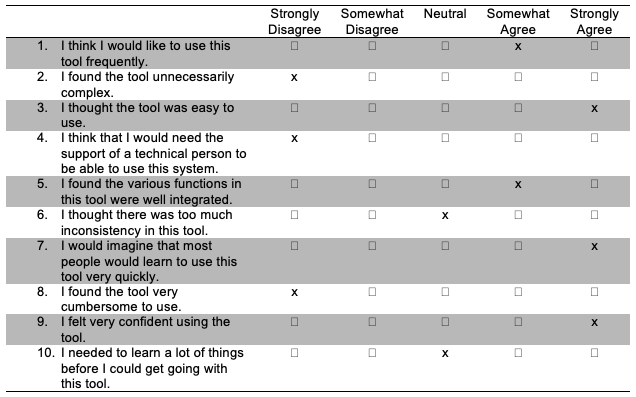
\includegraphics[width=0.95\textwidth]{graphics/sus_person6.png}
\end{center}

\textbf{Follow-up:}  
\begin{enumerate}
    \item \textbf{Was hat Ihnen am Tool am besten gefallen?}
    \begin{itemize}
        \item Möglichkeit kreativ zu sein.
    \end{itemize}

    \item \textbf{Gab es etwas, das verwirrend oder schwierig zu bedienen war?}
    \begin{itemize}
        \item Kurz verwirrt/irritiert, weil Wand „mitgegümmelt“ wurde.
    \end{itemize}

    \item \textbf{Fehlt etwas, das Sie erwartet oder gerne gehabt hätten? / Verbesserungsvorschläge}
    \begin{itemize}
        \item Bessere Stiftspitze (spitzer).  
        \item Anmerkung: Beamer-Qualität beachten.  
        \item Hintergrund nicht mit „gümmeln“, abhängig von Ausgangslage.  
        \item Feinerer Stiftkopf beim weissen Stift besser als beim schwarzen.  
        \item Sichtbarkeit der Taskleiste verwirrend (dachte, etwas aus Windows File Explorer holen zu müssen).  
        \item Gitternetz am Anfang unklar, ob man daran gebunden ist oder darüber hinaus malen kann.  
        \item Bei weiteren Tests am Anfang mehr Einweisung geben, damit Personen besseres Gefühl haben.
    \end{itemize}
\end{enumerate}

\clearpage



\end{appendix}


%%---NOTES for DEBUG---------------------------------------------------------------------
%\newpage
%\listoftodos[\section{Todo-Notes}]
%\clearpage

\end{document}